%!TEX program = xelatex
\documentclass[dvipsnames, svgnames,a4paper,11pt]{article}
% ----------------------------------------------------
%   中山大学物理与天文学院本科实验报告模板
%   作者:Huanyu Shi,2019级
%   知乎:https://www.zhihu.com/people/za-ran-zhu-fu-liu-xing
%   Github:https://github.com/huanyushi/SYSU-SPA-Labreport-Template
%   Last update : 2023.4.10
% ----------------------------------------------------

% ----------------------------------------------------- 
%	加边框的命令
%	参考:https://tex.stackexchange.com/questions/531559/how-to-add-the-page-border-for-first-two-pages-in-latex
\usepackage{tikz}
\usetikzlibrary{calc}
\usepackage{eso-pic}
\AddToShipoutPictureBG{%
\begin{tikzpicture}[overlay,remember picture]
\draw[line width=0.6pt] % 边框粗细
    ($ (current page.north west) + (0.6cm,-0.6cm) $)
    rectangle
    ($ (current page.south east) + (-0.6cm,0.6cm) $); % 边框位置
\end{tikzpicture}}


\usepackage{xcolor}
\definecolor{c1}{HTML}{2752C9} % 目录颜色
\definecolor{c2}{RGB}{190,20,83} % 引用颜色

\usepackage{ctex}
\usepackage[top=28mm,bottom=28mm,left=15mm,right=15mm]{geometry}
\usepackage{hyperref} 
\hypersetup{
	colorlinks,
	linktoc = section, % 超链接位置,选项有section, page, all
	linkcolor = c1, % linkcolor 目录颜色
	citecolor = c1  % citecolor 引用颜色
}
\usepackage{amsmath,enumerate,multirow,float}
\usepackage{tabularx}
\usepackage{tabu}
\usepackage{subfig}
\usepackage{fancyhdr}
\usepackage{graphicx}
\usepackage{wrapfig}  
\usepackage{physics}
\usepackage{appendix}
\usepackage{amsfonts}

%
\usepackage{tcolorbox}
\tcbuselibrary{skins,breakable}
\newtcolorbox{tbox}[2][]{
    colframe=black!70!,
    breakable,
    enhanced,
	boxrule =0.5pt,
    title = {#2},
    fonttitle = \large\kaishu\bfseries,
	drop fuzzy shadow,
    #1
}
\newtcolorbox[auto counter,number within=section]{question}[1][]{
  top=2pt,bottom=2pt,arc=1mm,
  boxrule=0.5pt,
%   frame hidden,
  breakable,
  enhanced, %跨页后不会显示下边框
  coltitle=c1!80!gray,
  colframe=c1,
  colback=c1!3!white,
  drop fuzzy shadow,
  title={思考题~\thetcbcounter:\quad},
  fonttitle=\bfseries,
  attach title to upper,
  #1
}

% ---------------------------------------------------------------------
%	利用cleveref改变引用格式,\cref是引用命令
\usepackage{cleveref}
\crefformat{figure}{#2{\textcolor{c2}{图 #1}}#3} % 图片的引用格式
\crefformat{equation}{#2{(\textcolor{c2}{#1})}#3} % 公式的引用格式
\crefformat{table}{#2{\textcolor{c2}{表 #1}}#3} % 表格的引用格式


% ---------------------------------------------------------------------
%	页眉页脚设置
\fancypagestyle{plain}{\pagestyle{fancy}}
\pagestyle{fancy}
\lhead{\kaishu 中山大学物理与天文学院近代物理实验\uppercase\expandafter{\romannumeral1}} % 左边页眉,学院 + 课程
\rhead{\kaishu D8 \quad 氦氖激光综合实验} % 右边页眉,实验报告标题
\cfoot{\thepage} % 页脚,中间添加页码


% ---------------------------------------------------------------------
%	对目录、章节标题的设置
\renewcommand{\contentsname}{\centerline{\huge 目录}}
\usepackage{titlesec}
\usepackage{titletoc}
% \titleformat{章节}[形状]{格式}{标题序号}{序号与标题间距}{标题前命令}[标题后命令]
\titleformat{\section}{\centering\LARGE\songti}{}{1em}{}

% ---------------------------------------------------------------------
%   listing代码环境设置
\usepackage{listings}
\lstloadlanguages{python}
\lstdefinestyle{pythonstyle}{
backgroundcolor=\color{gray!5},
language=python,
frameround=tftt,
frame=shadowbox, 
keepspaces=true,
breaklines,
columns=spaceflexible,                   
basicstyle=\ttfamily\small, % 基本文本设置,字体为teletype,大小为scriptsize
keywordstyle=[1]\color{c1}\bfseries, 
keywordstyle=[2]\color{Red!70!black},   
stringstyle=\color{Purple},       
showstringspaces=false,
commentstyle=\ttfamily\scriptsize\color{green!40!black},%注释文本设置,字体为sf,大小为smaller
tabsize=2,
morekeywords={as},
morekeywords=[2]{np, plt, sp},
numbers=left, % 代码行数
numberstyle=\it\tiny\color{gray}, % 代码行数的数字字体设置
stepnumber=1,
rulesepcolor=\color{gray!30!white}
}




% ---------------------------------------------------------------------
%	其他设置
\def\degree{${}^{\circ}$} % 角度
\graphicspath{{./images/}} % 插入图片的相对路径
\allowdisplaybreaks[4]  %允许公式跨页 % 导入模板的相关设置
\usepackage{lipsum}
\usepackage{enumitem}
\usepackage{tabularray}  %绘制表格时可以更加方便添加框线
\setlist[enumerate]{label=\textup{(\arabic*)}}



%---------------------------------------------------------------------
%	正文
%---------------------------------------------------------------------

\begin{document}


\begin{table}
	\renewcommand\arraystretch{1.7}
	\begin{tabularx}{\textwidth}{
		|X|X|X|X
		|X|X|X|X|}
	\hline
	\multicolumn{2}{|c|}{预习报告}&\multicolumn{2}{|c|}{实验记录}&\multicolumn{2}{|c|}{分析讨论}&\multicolumn{2}{|c|}{总成绩}\\
	\hline
	\LARGE25 & & \LARGE30 & & \LARGE25 & & \LARGE80 & \\
	\hline
	\end{tabularx}
\end{table}


\begin{table}
	\renewcommand\arraystretch{1.7}
	\begin{tabularx}{\textwidth}{|X|X|X|X|}
	\hline
	专业:& 物理学 &年级:& 2022级\\
	\hline
	姓名:& 戴鹏辉  & 学号: & 2344016 \\
	\hline
	日期:& 2024/9/23 & 教师签名:& \\
	\hline
	\end{tabularx}
\end{table}

\begin{center}
	\LARGE D3 \quad 量子密钥分发
\end{center}

\textbf{【实验报告注意事项】}
\begin{enumerate}
	\item 实验报告由三部分组成:
	\begin{enumerate}
		\item 预习报告:(提前一周)认真研读\underline{\textbf{实验讲义}},弄清实验原理;实验所需的仪器设备、用具及其使用(强烈建议到实验室预习),完成课前预习思考题;了解实验需要测量的物理量,并根据要求提前准备实验记录表格(第一循环实验已由教师提供模板,可以打印)。预习成绩低于10分(共20分)者不能做实验。
	    \item 实验记录:认真、客观记录实验条件、实验过程中的现象以及数据。实验记录请用珠笔或者钢笔书写并签名(\textcolor{red}{\textbf{用铅笔记录的被认为无效}})。\textcolor{red}{\textbf{保持原始记录,包括写错删除部分,如因误记需要修改记录,必须按规范修改。}}(不得输入电脑打印,但可扫描手记后打印扫描件);离开前请实验教师检查记录并签名。
	    \item 分析讨论:处理实验原始数据(学习仪器使用类型的实验除外),对数据的可靠性和合理性进行分析;按规范呈现数据和结果(图、表),包括数据、图表按顺序编号及其引用;分析物理现象(含回答实验思考题,写出问题思考过程,必要时按规范引用数据);最后得出结论。
	\end{enumerate}
	\textbf{实验报告就是将预习报告、实验记录、和数据处理与分析合起来,加上本页封面。}
	% \item 每次完成实验后的一周内交\textbf{实验报告}(特殊情况不能超过两周)。
	\item 实验报告注意事项
		\begin{enumerate}[label=\roman*.]
			\item 系统工作温度在 15°-30°的环境中,尤其避免过高温度下使用本系统。
			\item 实验元件会单独给出,实验前检查是否完整。除给出的元件外,整体密钥分发系统不要触碰。
			\item 镜筒等光机械安装时,螺丝拧紧避免晃动。光机械元件的调节旋钮,安装前,将螺丝行程旋至中间位置,方便实验过程中调节。
			\item 所有镜片避免用手接触光学面,拿捏过程中,光学面垂直于平台,避免灰尘,使用完收入对应的盒子中。安装镜片需靠近台面,避免镜片跌落摔碎。
			\item \textcolor{red}{请不要打开单光子探测器的黑色遮盖物。}
			\item \textcolor{red}{不要使眼睛与光路处于同一水平面,不要用手直接接触激光,激光为 30mw 紫外激光,必须戴好护目镜。}
		\end{enumerate}
\end{enumerate}


\clearpage
\tableofcontents
\clearpage

\setcounter{section}{0}
\section{D3 \quad 量子密钥分发 \quad\heiti 预习报告}
	
\subsection{实验目的}
\begin{enumerate}
	\item 掌握控制和测量光子的偏振;
	\item 掌握单光子的标定;
	\item 掌握单光子的探测及相应探测器效率的测量;
	\item 掌握 BB84 量子密钥分发过程的数据处理。
	
\end{enumerate}

\subsection{仪器用具}
\begin{table}[htbp]
	\centering
	\renewcommand\arraystretch{1.6}
	% \setlength{\tabcolsep}{10mm}
	\caption{偏振测量实验}
	\begin{tabular}{p{0.05\textwidth}|p{0.20\textwidth}|p{0.05\textwidth}|p{0.5\textwidth}}
		\hline
		编号& 仪器用具名称 & 数量 &  主要参数(型号,测量范围,测量精度等) \\
		\hline
		1	&	准直激光器 	& 1 & 波长:404nm,最大功率:150mW\\

		2	&	偏振分光棱镜 	& 2 & 波长:404nm,消光比>500	 \\
		
		3	&	半波片 & 2 &	波长:404nm,零级 	\\
		
		4	&	小型磁性底座	&  & MB105	\\
		
		5	&	PH 系列杆架	& 6 & PH102	\\

		6	&	SP 系列接杆	& 6 & SP104 \\

		7	&	激光器镜架	& 6 & OM311	\\

		8	&	精密棱镜台	& 2 & PPM101	\\

		9	&	偏光镜架	& 2 & PM101	\\

		10	&	可见光功率计& 2 & PM100、S120VC	\\

		11	&	直流稳压电源& 1 & GPD-3303D	\\
		\hline
	\end{tabular}
	\label{tbl:偏振测量实验}
\end{table}

\begin{table}[htbp]
	\centering
	\renewcommand\arraystretch{1.6}
	% \setlength{\tabcolsep}{10mm}
	\caption{单光子标定的用具}
	\begin{tabular}{p{0.05\textwidth}|p{0.20\textwidth}|p{0.05\textwidth}|p{0.5\textwidth}}
		\hline
		编号& 仪器用具名称 & 数量 &  主要参数(型号,测量范围,测量精度等) \\
		\hline
		1	&	密钥分发系统 	& 1 & 波长:404nm	\\

		2	&	可见光功率计 	& 1 & PM100、S120VC	 \\
		\hline
	\end{tabular}
	\label{tbl:单光子标定的用具}

\end{table}

\begin{table}[htbp]
	\centering
	\renewcommand\arraystretch{1.6}
	% \setlength{\tabcolsep}{10mm}
	\caption{单光子的探测及相应探测器探测效率测量的用具}
	\begin{tabular}{p{0.05\textwidth}|p{0.20\textwidth}|p{0.05\textwidth}|p{0.5\textwidth}}
		\hline
		编号& 仪器用具名称 & 数量 &  主要参数(型号,测量范围,测量精度等) \\
		\hline
		1	&	反射镜 	& 1 & 波长:404nm,45 度入射	\\

		2	&	滤波片 	& 1 & 波长:405nm,带宽:3nm	 \\
		
		3	&	光纤准直器 & 1 &	F671FC-405 	\\
		
		4	&	反射镜折叠架	& 1 & OM402	\\
		
		5	&	透镜固定架	& 1 & LH102	\\

		6	&	光纤耦合架	& 1 & PFC201 \\

		7	&	小型磁性底座	& 3 & MB105	\\

		8	&	PH 系列杆架	& 3 & PH102	\\

		9	&	SP 系列接杆	& 1 & SP104	\\

		10	&	SP 系列接杆	& 2	& SP134	\\

		11	&	可见光功率计	& 1 & PM100、S120VC	\\

		12	&	直流稳压电源& 1 & GPD-3303D	\\
		\hline
	\end{tabular}
	\label{tbl:单光子的探测及相应探测器探测效率测量的用具}

\end{table}


\begin{table}[htbp]
	\centering
	\renewcommand\arraystretch{1.6}
	% \setlength{\tabcolsep}{10mm}
	\caption{密钥分发过程数据处理的用具}
	\begin{tabular}{p{0.05\textwidth}|p{0.20\textwidth}|p{0.05\textwidth}|p{0.5\textwidth}}
		\hline
		编号& 仪器用具名称 & 数量 &  主要参数(型号,测量范围,测量精度等) \\
		\hline
		1	&	密钥分发系统 	& 1 & 波长:404nm	\\
		\hline
	\end{tabular}
	\label{tbl:密钥分发过程数据处理的用具}

\end{table}

\clearpage

\subsection{原理概述}

	\begin{itemize}
		\item \textbf{量子密钥分发的基本原理}:
		\begin{itemize}
			\item 量子密钥分发(Quantum Key Distribution, QKD)是一种利用量子力学基本原理进行密钥分发的方法,主要解决经典密码体系中密钥安全分发的问题。QKD的安全性并不是依赖算法复杂性,而是基于量子力学的物理定律,如测量塌缩理论、海森堡不确定原理和量子不可克隆定律。这些定律确保了任何窃听行为都会干扰量子态,从而被合法通信双方检测到。
			\item QKD采用单光子作为信息的物理载体,单光子是光场的最小能量单元,具有不可分割性;单光子的量子态不可克隆,无法通过一次测量完全准确地复制单光子的状态;测量单光子的偏振态具有概率性,测量结果依赖于量子态处于测量算子的本征态时才能精确获得。
		\end{itemize}
		
		\item \textbf{BB84协议的工作原理}:
		\begin{itemize}
			\item BB84协议是最早提出的QKD协议,利用光子的偏振态来编码信息。光子的偏振态随机选自两个基:水平/垂直基($\oplus$基)和对角基($\otimes$基)。在通信中,发送方(Alice)随机选择基和态来制备光子并发送给接收方(Bob)。
			\item Bob接收到光子后,也随机选择一个基进行测量。由于Bob的基选择是随机的,只有当测量基与Alice的制备基一致时,Bob的测量结果才是有意义的;当基不同时,测量结果无效。
			\item Alice和Bob在公开信道上公布各自的基的选择,而不公布测量结果,仅保留基相同的测量结果用于密钥生成。这种随机选择和匹配的机制使得窃听者难以获取信息,因为窃听者的任何测量都会引入错误,并被Alice和Bob检测到。
		\end{itemize}

		\item \textbf{QKD的安全性基础}:
		\begin{itemize}
			\item 单光子态的不可分割性和不可克隆性使得窃听者无法在不被发现的情况下复制或测量这些光子。
			\item 在BB84协议中,如果窃听者试图测量光子状态,其随机选择的测量基可能与Alice的基不匹配,从而干扰量子态,导致误码率增加。Alice和Bob通过检测误码率来判断是否存在窃听,当误码率超过安全阈值时,说明存在窃听行为。
			\item QKD的安全性是信息论上的无条件安全,即只要误码率低于一定阈值,通过后续的纠错和隐私放大步骤,Alice和Bob可以提取出无条件安全的共享密钥。
		\end{itemize}
	\end{itemize}
	




\subsection{实验前思考题}

% 思考题1
\begin{question}
	回顾偏振光实验,说明$\lambda / 2$波片,$\lambda / 4$波片的工作原理;
\end{question}


	晶体介质的折射率与光波的偏振方向有关,是各向异性的。当晶体介质的折射率在两个方向上不同时,分别记作$n_x$和$n_y$,且$n_x>n_y$时,可以定义两个方向上的相位速度$c_x$和$c_y$,其中$c_x<c_y$。晶体中的$x$轴被称为慢轴,$y$轴被称为快轴。在晶体中,一条折射线总符合普通的折射定律,称作寻常光(或o光),而另一条折射线不遵守普通的折射定律,称作非常光(或e光)。o光和e光都是偏振光,且两光束的振动方向相互垂直。

	因为通过该偏振片导致$x$和$y$方向偏振光的光程差为:$\delta=(n_x-n_y)d$,$d$为偏振片厚度。

	\begin{enumerate}
		\item $\lambda/ 2$波片指,对于一个给定的波长$\lambda$平行光正入射波晶片时, o光和e光的光程差$\delta=\frac{\lambda}{2}$。
		另外, $\lambda/ 2$波片是对特定波长的光通过,否则没有任何意义。
		
		若线偏振光经过$\lambda/ 2$波片,出射光还是线偏振光,但相对于o轴或e轴对称。特别的,平行于o轴或e轴入射的偏振光,经过波片后方向保持不变。
		
		若椭圆偏振光经过$\lambda/ 2$波片,出射光仍是椭圆偏振光,但旋转方向相反。

		\item $\lambda/ 4$波片指,对于一个给定的波长$\lambda$平行光正入射波晶片时, o光和e光的光程差$\delta=\frac{\lambda}{4}$。
		同样的, $\lambda/ 4$波片是对特定波长的光通过,否则没有任何意义。

		线偏振光通过$\lambda/ 4$波片后,当入射角为0°、90°、180°、270°时,出射光仍然是线偏振光。\\
		当入射角为45°、135°、225°、315°时,出射光变为圆偏振光。\\
		对于其他入射角度,出射光为椭圆偏振光。


	\end{enumerate}


% 思考题2
\begin{question}
	如何检测一个任意方向的线偏振光?
\end{question}

	通过使用线偏振片和光功率计,可实现任意方向的线偏振光的检测,具体方法如下:

	\begin{enumerate}
		\item 将一个线偏振片置于入射光路中,并让光通过该线偏振片。
		\item 缓慢旋转线偏振片,记录光强随角度的变化。检测器记录透过偏振片的光强度 \( I \)。
		\item 当透过光强达到最大值时,说明此时线偏振片的偏振方向与入射线偏振光的偏振方向平行;
		
		当透过光强达到最小值(理论上为零)时,线偏振片的偏振方向与入射线偏振光的偏振方向垂直。

		具体的数学关系可以用马吕斯定律(Malus's Law)描述:
		\[
			I = I_0 \cos^2 \theta
		\]

		其中 \( I \) 为透过偏振片的光强,\( I_0 \) 为入射光强,\( \theta \) 为入射光的偏振方向与偏振片方向之间的夹角。

	\end{enumerate}


	




% 思考题3
\begin{question}
	单光子为什么不能直接用普通功率计测量?
\end{question}

	单光子不能直接用普通功率计测量,主要原因如下:

	\begin{enumerate}
		\item \textbf{功率计的灵敏度不足:}普通功率计通常用于测量宏观光强(如mW或W级别),它们的探测器需要足够多的光子来产生可测的电信号;而单光子的能量极其微小,通常在eV量级,对普通功率计来说,这样的能量远低于其探测阈值,导致无法检测单光子事件。
		\item \textbf{响应时间和噪声问题:}普通功率计的响应时间较长且噪声较大,难以分辨单个光子的到达。单光子事件发生的时间间隔可能非常短,并且在单光子水平下,信号很容易被背景噪声淹没。
		\item \textbf{检测原理不同:}普通功率计测量的是光的平均功率,通过探测大量光子的累积效应获得信号。单光子测量需要通过专门设计的单光子探测器(如光电倍增管、雪崩光电二极管或超导纳米线单光子探测器),这些探测器能够在单光子事件发生时产生响应,记录单个光子的到达时间和数量。
		\item \textbf{量子效率和探测机制:}普通功率计的量子效率通常较低,对单光子的探测效率不足。而单光子探测器则设计有高量子效率,能够可靠地探测并计数单个光子。
	\end{enumerate}





% 思考题4
\begin{question}
	检验单光子探测器的探测效率可以用强光吗?
\end{question}

	不可直接使用强光,因为单光子探测器设计用于探测极低光强度下的单光子事件。使用强光源可能会导致以下问题:

	\begin{enumerate}
		\item \textbf{饱和效应:}单光子探测器的探测机制是基于对单个光子的响应设计的。当入射光强度过高时,探测器会进入饱和状态,无法区分单个光子事件,导致信号失真,并且探测效率测量不准确。
		\item \textbf{探测器损坏风险:}单光子探测器通常具有较高的增益,用于放大微弱的单光子信号。强光会产生过大的电流,可能会损坏探测器的电子元件或造成永久性损坏。
		\item \textbf{非线性响应:}单光子探测器在强光下的响应不再是线性的,这与单光子探测的条件不符,导致效率评估失真。探测效率是定义在单光子条件下的,即探测器对单个光子的响应概率。
	\end{enumerate}
	

	正确的探测效率检验方法
	检验单光子探测器的探测效率一般采用低强度的光源,保证光强度足够低,使得光子事件是稀疏的且近似服从泊松分布。具体步骤如下:

	\begin{enumerate}
		\item \textbf{使用弱光源:}使用经过强度衰减的激光器或 LED,光强控制在单光子水平上。通常通过中性密度滤光片或分束器来精确控制光子的通量。
		\item \textbf{参考探测器:}使用已知效率的标准探测器或计数装置作为参考,与待测单光子探测器同时测量同一光源的光子通量。
		\item \textbf{统计计数事件:}记录单光子探测器和参考探测器在相同条件下的响应事件数量,通过比较计数来计算单光子探测器的探测效率。
		\item \textbf{量子效率计算:}探测效率(量子效率)定义为探测到的光子数与实际入射光子数之比。
	\end{enumerate}

	使用弱光源和统计方法能够精确测量单光子探测器的探测效率,确保测量结果的准确性。




% 思考题5
\begin{question}
	BB84 协议的原理和步骤。
\end{question}

	\begin{itemize}
		\item \textbf{BB84协议的基本原理}:
		\begin{itemize}
			\item BB84协议利用了量子态不可克隆原理和测量干扰原理。在量子通信中,量子比特(qubit)不能被精确复制,并且任何对量子态的测量都会不可避免地对量子态产生干扰。因此,窃听者试图在通信过程中窃听信息时,必然会在数据中留下痕迹,这些痕迹可以被通信双方检测到。
		\end{itemize}
		
		\item \textbf{BB84协议的步骤}:
		\begin{enumerate}
			\item \textbf{量子态编码}:
			\begin{itemize}
				\item 通信双方称为发送者Alice和接收者Bob。Alice随机选择两种基和两个状态来发送比特。
				\item Alice使用两种正交基态来编码信息:
				\begin{itemize}
					\item 直角基($\oplus$基): $\{|0\rangle, |1\rangle\}$
					\item 对角基($\otimes$基): $\{|+\rangle = \frac{|0\rangle + |1\rangle}{\sqrt{2}}, |-\rangle = \frac{|0\rangle - |1\rangle}{\sqrt{2}}\}$
				\end{itemize}
				\item Alice随机选择这些基态中的一个,来表示经典比特0或1。例如:
				\begin{itemize}
					\item 用$\oplus$基的$|0\rangle$表示比特0,用$\oplus$基的$|1\rangle$表示比特1。
					\item 用$\otimes$基的$|+\rangle$表示比特0,用$\otimes$基的$|-\rangle$表示比特1。
				\end{itemize}
			\end{itemize}

			\item \textbf{量子态传输}:
			\begin{itemize}
				\item Alice将随机选择的量子态发送给Bob。由于量子态的不可克隆性,Eve无法准确复制或窃听而不被察觉。
			\end{itemize}

			\item \textbf{基的选择与测量}:
			\begin{itemize}
				\item Bob在接收到量子态后,随机选择$\oplus$基或$\otimes$基对每个光子进行测量。由于Bob的基选择是随机的,测量结果在Alice的基与Bob的基相同时是正确的,在基不同的时候则是随机的。
			\end{itemize}

			\item \textbf{基的公布与筛选}:
			\begin{itemize}
				\item Alice和Bob通过经典通信渠道(可以公开,但不保密)公布他们选择的基,\textbf{但不公布测量结果}。然后,他们保留那些在基选择相同的情况下的测量结果,丢弃基不同的测量结果。
			\end{itemize}

			\item \textbf{错误率检查}:
			\begin{itemize}
				\item Alice和Bob各自拥有一组相同基的比特序列,为了检测是否有窃听者存在,他们随机选择一部分比特进行比较。如果误码率低于一定阈值(通常设定在11\%以内),则说明没有明显的窃听,或者说窃听干扰较小,可以认为是安全的;如果误码率过高,则表明可能存在窃听,他们会丢弃这些密钥并重新开始协议。
			\end{itemize}

			\item \textbf{密钥提纯和隐私放大}:
			\begin{itemize}
				\item Alice和Bob根据检测到的错误率,使用纠错和隐私放大技术来去除误差和窃听者可能获取的信息,生成一个更短但更安全的密钥。
			\end{itemize}

			\item \textbf{共享密钥的生成}:
			\begin{itemize}
				\item 经过上述步骤后,Alice和Bob共享一条安全密钥,可以用于后续的加密通信。
			\end{itemize}
		\end{enumerate}

		\item \textbf{BB84协议的安全性}:
		\begin{itemize}
			\item BB84协议的安全性来自于量子测量的不可逆性和不可克隆定理:任何第三方在尝试窃听量子信道时,必然会干扰量子态,从而导致测量误差。这些误差可以被Alice和Bob检测到,从而保证密钥分发的安全性。即便第三方窃听了经典通信信道,由于该信道上不传输实际密钥值,仅基的选择信息,因此不会危及密钥的安全性。
			\item BB84协议是量子密码学的基础,广泛用于研究和实际应用中,确保通信安全性。
		\end{itemize}
	\end{itemize}





% 思考题6
\begin{question}
	密钥分发过程中,为什么需要有同步信号?
\end{question}

	\begin{itemize}
		\item 在量子密钥分发过程中,特别是在BB84协议中,同步信号的作用至关重要。具体原因如下:
		
		\begin{enumerate}
			\item \textbf{确保接收者正确接收每个量子态:}  
			在量子密钥分发过程中,发送方(Alice)会按照一定的时间顺序发送一系列量子态给接收方(Bob)。同步信号用于确保Bob在正确的时间窗口内进行测量,这样他能够与Alice发送的量子态一一对应。如果没有同步信号,Bob可能会在错误的时刻进行测量,从而导致数据对不上,增加误码率。

			\item \textbf{减少测量误差和丢包率:}  
			如果发送和接收没有时间上的同步,量子态可能在Bob还未准备好时就已经发出或者被测量,导致测量失败或丢失。这会增加数据损失,降低密钥生成效率。而同步信号可以帮助双方在测量时刻上匹配,减少测量误差和丢包率。

			\item \textbf{避免干扰和重叠:}  
			没有同步信号时,不同量子态之间可能会发生重叠或干扰,尤其是在高速传输的情况下。同步信号确保每个量子态在独立的时间窗口内被测量,避免相邻态之间的干扰,保证密钥分发的准确性。

			\item \textbf{提高协议效率:}  
			通过同步信号,Alice和Bob可以协调他们的设备运行在相同的时间步伐下,最大限度地提高密钥分发速率。否则,由于不匹配的时序问题,可能会频繁出现测量空闲或无效的情况,降低系统整体效率。

			\item \textbf{检测和对抗窃听:}  
			时间同步能够提高对潜在窃听者的检测能力。如果窃听者试图在信道中插入或篡改数据,同步不当可能会导致显著的误码率上升,从而暴露窃听行为。通过同步,Alice和Bob更容易检测到任何异常的时序变化。
		\end{enumerate}

		% \item 因此,同步信号在量子密钥分发中至关重要,保证了数据传输的准确性、稳定性和安全性。
	\end{itemize}


\clearpage
\begin{table}
	\renewcommand\arraystretch{1.7}
	\centering
	\begin{tabularx}{\textwidth}{|X|X|X|X|}
	\hline
	专业:& 物理学 &年级:& 2022级 \\
	\hline
	姓名:& 戴鹏辉 & 学号:& 22344016 \\
	\hline
	室温:& 26℃ & 实验地点: & A102 \\
	\hline
	学生签名:& 
\includegraphics[width=0.9in]{name-TaLEs.jpg} & 评分: &\\
	\hline
	实验时间:& 2024/09/27& 教师签名:&\\
	\hline
	\end{tabularx}
\end{table}

\section{D3 \quad 量子密钥分发 \quad\heiti 实验记录}

\subsection{实验内容和步骤}

	\subsubsection{实验一 \quad 光的偏振的测量和控制}

		% dBm为分贝毫瓦,计算公式为
		% \[
		% 	x \equiv 10 \log \frac{P(\mathrm{mW})}{1 \mathrm{mW}}
		% \]
	
		\begin{enumerate}
			\item 将光学元件按照“Laser - PBS1 - 光功率计”的顺序摆放,测量激光器通过PBS1后的反射功率和透射功率。测量数据如\cref{tbl:D3-1-1}所示。
			
				\begin{table}[htbp]
					\centering
					\begin{tabular}{|c|c|cc|} 
					\hline
					序号 & 名称              & 数据    & 单位   \\ 
					\hline
					1  & Laser+PBS1 反射功率 & 9.12  & dBm  \\
					2  & Laser+PBS1 透射功率 & 15.05 & dBm  \\
					\hline
					\end{tabular}
					\caption{激光器通过PBS1后的反射功率和透射功率}
					\label{tbl:D3-1-1}
				\end{table}


			
			\item 在上一步的基础上,在“Laser”和“PBS1”之间加入一个半波片“HWP1”,旋转HWP1,测量激光器通过PBS1后的最大、最小透射功率和最大、最小的反射功率,结果如\cref{tbl:D3-1-2}所示。
				
				\begin{table}[htbp]
					\centering
					\begin{tabular}{|c|c|cc|} 
					\hline
					序号 & 名称                       & 数据    & 单位   \\ 
					\hline
					1  & Laser + HWP1+PBS1 最大反射功率 & 15.88 & dBm  \\
					2  & Laser + HWP1+PBS1 最大透射功率 & 15.8  & dBm  \\
					3  & Laser + HWP1+PBS1 最小反射功率 & -1.66 & dBm  \\
					4  & Laser + HWP1+PBS1 最小透射功率 & -8.42 & dBm  \\
					\hline
					\end{tabular}
					\caption{加入半波片后,激光器通过PBS1后的反射功率和透射功率}
					\label{tbl:D3-1-2}
				\end{table}
			
			\item 将光学元件按照“Laser - PBS1 - HWP1 - PBS2 - 光功率计”的顺序摆放,旋转HWP1,测量激光器通过PBS2后的功率变化,结果如\cref{tbl:D3-1-3}所示。
			
				\begin{table}[htbp]
					\centering
					\begin{tblr}{
					cells = {c},
					cell{1}{2} = {c=2}{},
					vline{1-4,6} = {1}{},
					vline{1-2,4,6} = {2-18}{},
					hline{1-2,19} = {-}{},
					}
					序号 & 名称              &           & 数据     & 单位  \\
					1  & 半波片 1 转动 0°     & PBS2 透射功率 & -28.79 & dBm \\
					2  & 半波片 1 转动 22.5°  & PBS2 透射功率 & -5.44  & dBm \\
					3  & 半波片 1 转动 45°    & PBS2 透射功率 & -2.36  & dBm \\
					4  & 半波片 1 转动 67.5°  & PBS2 透射功率 & -5.72  & dBm \\
					5  & 半波片 1 转动 90°    & PBS2 透射功率 & -24.06 & dBm \\
					6  & 半波片 1 转动 112.5° & PBS2 透射功率 & -5.65  & dBm \\
					7  & 半波片 1 转动 135°   & PBS2 透射功率 & -2.55  & dBm \\
					8  & 半波片 1 转动 157.5° & PBS2 透射功率 & -4.88  & dBm \\
					9  & 半波片 1 转动 180°   & PBS2 透射功率 & -24.6  & dBm \\
					10 & 半波片 1 转动 202.5° & PBS2 透射功率 & -5.02  & dBm \\
					11 & 半波片 1 转动 225°   & PBS2 透射功率 & -2.35  & dBm \\
					12 & 半波片 1 转动 247.5° & PBS2 透射功率 & -6.53  & dBm \\
					13 & 半波片 1 转动 270°   & PBS2 透射功率 & -21.65 & dBm \\
					14 & 半波片 1 转动 292.5° & PBS2 透射功率 & -5.68  & dBm \\
					15 & 半波片 1 转动 315°   & PBS2 透射功率 & -2.03  & dBm \\
					16 & 半波片 1 转动 337.5° & PBS2 透射功率 & -5.13  & dBm \\
					17 & 半波片 1 转动 360°   & PBS2 透射功率 & -27.92 & dBm 
					\end{tblr}
					\caption{透射功率随HWP1的变化}
					\label{tbl:D3-1-3}
				\end{table}
			  
			
			
			\item 将光学元件按照“Laser - PBS1 - HWP1 - HWP2 - PBS2 - 光功率计”的顺序摆放,光路图如\cref{fig:D3-1-2}所示。首先将HWP1调整至光轴竖直(在上一步以确定光轴位置),然后旋转HWP2,测量激光器通过PBS2后的功率变化,结果如\cref{tbl:D3-1-4}所示。
			
				\begin{figure}[htbp]
					\centering
					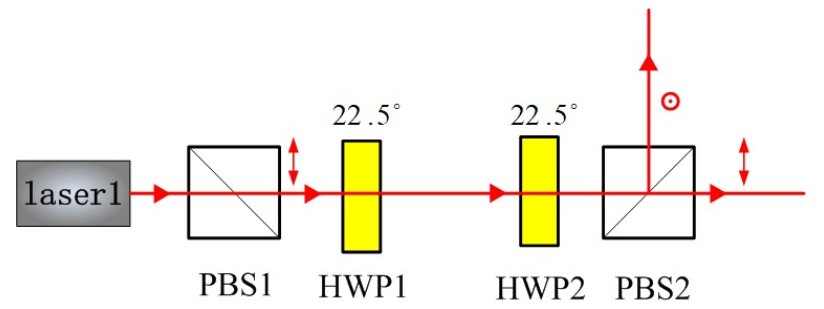
\includegraphics[width=0.9\textwidth]{D3-1-2.png}
					\caption{第四步的光路图}
					\label{fig:D3-1-2}
				\end{figure}
				
				

				
				\begin{table}[htbp]
					\centering
					\begin{tblr}{
					cells = {c},
					cell{1}{2} = {c=2}{},
					vline{1-4,6} = {1}{},
					vline{1-2,4,6} = {2-18}{},
					hline{1-2,19} = {-}{},
					}
					序号 & 名称              &           & 数据     & 单位  \\
					1  & 半波片 2 转动 0°     & PBS2 透射功率 & -25.32 & dBm \\
					2  & 半波片 2 转动 22.5°  & PBS2 透射功率 & 10.56  & dBm \\
					3  & 半波片 2 转动 45°    & PBS2 透射功率 & 13.65  & dBm \\
					4  & 半波片 2 转动 67.5°  & PBS2 透射功率 & 11.68  & dBm \\
					5  & 半波片 2 转动 90°    & PBS2 透射功率 & -11.2  & dBm \\
					6  & 半波片 2 转动 112.5° & PBS2 透射功率 & 10.74  & dBm \\
					7  & 半波片 2 转动 135°   & PBS2 透射功率 & 14.07  & dBm \\
					8  & 半波片 2 转动 157.5° & PBS2 透射功率 & 9.49   & dBm \\
					9  & 半波片 2 转动 180°   & PBS2 透射功率 & -24.2  & dBm \\
					10 & 半波片 2 转动 202.5° & PBS2 透射功率 & 11.16  & dBm \\
					11 & 半波片 2 转动 225°   & PBS2 透射功率 & 14.03  & dBm \\
					12 & 半波片 2 转动 247.5° & PBS2 透射功率 & 11.02  & dBm \\
					13 & 半波片 2 转动 270°   & PBS2 透射功率 & -12.71 & dBm \\
					14 & 半波片 2 转动 292.5° & PBS2 透射功率 & 11.06  & dBm \\
					15 & 半波片 2 转动 315°   & PBS2 透射功率 & 14.13  & dBm \\
					16 & 半波片 2 转动 337.5° & PBS2 透射功率 & 10.77  & dBm \\
					17 & 半波片 2 转动 360°   & PBS2 透射功率 & -18.45 & dBm 
					\end{tblr}
					\caption{透射功率随HWP2的变化}
					\label{tbl:D3-1-4}
				\end{table}

		\end{enumerate}



		实验一的数据记录如\cref{tbl:D3-1}所示。


			\begin{longtblr}[
				caption = {偏振控制和测量记录表格},  % 这里填写标题
    			label = {tbl:D3-1},  % 这里填写标签,用于引用
				% label = none,
				entry = none,
			  ]{
				cells = {c},
				cell{1}{2} = {c=2}{},
				cell{2}{2} = {c=2}{},
				cell{3}{2} = {c=2}{},
				cell{4}{2} = {c=2}{},
				cell{5}{2} = {c=2}{},
				cell{6}{2} = {c=2}{},
				cell{7}{2} = {c=2}{},
				vline{1-4,6} = {1-7}{},
				vline{1-2,4,6} = {8-43}{},
				hline{1-2,4,8,25,27,44} = {-}{},
			  }
			  序号 & 名称                       &           & 数据     & 单位  \\
			  1  & Laser+PBS1 反射功率          &           & 9.12   & dBm \\
			  2  & Laser+PBS1 透射功率          &           & 15.05  & dBm \\
			  1  & Laser + HWP1+PBS1 最大反射功率 &           & 15.88  & dBm \\
			  2  & Laser + HWP1+PBS1 最大透射功率 &           & 15.8   & dBm \\
			  3  & Laser + HWP1+PBS1 最小反射功率 &           & -1.66  & dBm \\
			  4  & Laser + HWP1+PBS1 最小透射功率 &           & -8.42  & dBm \\
			  1  & 半波片 1 转动 0°              & PBS2 透射功率 & -28.79 & dBm \\
			  2  & 半波片 1 转动 22.5°           & PBS2 透射功率 & -5.44  & dBm \\
			  3  & 半波片 1 转动 45°             & PBS2 透射功率 & -2.36  & dBm \\
			  4  & 半波片 1 转动 67.5°           & PBS2 透射功率 & -5.72  & dBm \\
			  5  & 半波片 1 转动 90°             & PBS2 透射功率 & -24.06 & dBm \\
			  6  & 半波片 1 转动 112.5°          & PBS2 透射功率 & -5.65  & dBm \\
			  7  & 半波片 1 转动 135°            & PBS2 透射功率 & -2.55  & dBm \\
			  8  & 半波片 1 转动 157.5°          & PBS2 透射功率 & -4.88  & dBm \\
			  9  & 半波片 1 转动 180°            & PBS2 透射功率 & -24.6  & dBm \\
			  10 & 半波片 1 转动 202.5°          & PBS2 透射功率 & -5.02  & dBm \\
			  11 & 半波片 1 转动 225°            & PBS2 透射功率 & -2.35  & dBm \\
			  12 & 半波片 1 转动 247.5°          & PBS2 透射功率 & -6.53  & dBm \\
			  13 & 半波片 1 转动 270°            & PBS2 透射功率 & -21.65 & dBm \\
			  14 & 半波片 1 转动 292.5°          & PBS2 透射功率 & -5.68  & dBm \\
			  15 & 半波片 1 转动 315°            & PBS2 透射功率 & -2.03  & dBm \\
			  16 & 半波片 1 转动 337.5°          & PBS2 透射功率 & -5.13  & dBm \\
			  17 & 半波片 1 转动 360°            & PBS2 透射功率 & -27.92 & dBm \\
			  1  & 放置半波片 1 且与光轴呈 22.5°      & PBS2 透射功率 & -5.44  & dBm \\
			  2  & 放置半波片 1 且与光轴呈 22.5°      & PBS2 反射功率 & -5.302 & dBm \\
			  1  & 半波片 2 转动 0°              & PBS2 透射功率 & -25.32 & dBm \\
			  2  & 半波片 2 转动 22.5°           & PBS2 透射功率 & 10.56  & dBm \\
			  3  & 半波片 2 转动 45°             & PBS2 透射功率 & 13.65  & dBm \\
			  4  & 半波片 2 转动 67.5°           & PBS2 透射功率 & 11.68  & dBm \\
			  5  & 半波片 2 转动 90°             & PBS2 透射功率 & -11.2  & dBm \\
			  6  & 半波片 2 转动 112.5°          & PBS2 透射功率 & 10.74  & dBm \\
			  7  & 半波片 2 转动 135°            & PBS2 透射功率 & 14.07  & dBm \\
			  8  & 半波片 2 转动 157.5°          & PBS2 透射功率 & 9.49   & dBm \\
			  9  & 半波片 2 转动 180°            & PBS2 透射功率 & -24.2  & dBm \\
			  10 & 半波片 2 转动 202.5°          & PBS2 透射功率 & 11.16  & dBm \\
			  11 & 半波片 2 转动 225°            & PBS2 透射功率 & 14.03  & dBm \\
			  12 & 半波片 2 转动 247.5°          & PBS2 透射功率 & 11.02  & dBm \\
			  13 & 半波片 2 转动 270°            & PBS2 透射功率 & -12.71 & dBm \\
			  14 & 半波片 2 转动 292.5°          & PBS2 透射功率 & 11.06  & dBm \\
			  15 & 半波片 2 转动 315°            & PBS2 透射功率 & 14.13  & dBm \\
			  16 & 半波片 2 转动 337.5°          & PBS2 透射功率 & 10.77  & dBm \\
			  17 & 半波片 2 转动 360°            & PBS2 透射功率 & -18.45 & dBm 
			  \end{longtblr}

	\subsubsection{实验二 \quad 单光子的探测及相应探测器效率的测量}
	\label{subsection2.1.2}

		\begin{enumerate}
			\item 理论计算,当到达单光子探测器的平均光子数为 0.1 光子/脉冲时,$\mathrm{LD_M}$ 和 $\mathrm{SPD_M}$ 之间需要多少衰减,计算过程如下:
				\begin{itemize}
					\item 单个 404 nm 光子的能量为:
						$$ E = h \nu = \frac{h c}{\lambda} = 6.626 \times 10^{-34} \times \frac{3 \times 10^{8}}{404 \times 10^{-9}} \mathrm{J} = 4.92 \times 10^{-19} \mathrm{J} $$

					\item 由于采用的 404nm 激光器的发光重复频率为 10MHz,因此,当到达$\mathrm{SPD_M}$的每个脉冲平均光子数为 0.1 个光子时,$\mathrm{SPD_M}$ 所探测到的功率为:
						\begin{align*}
							P = \mu \cdot f \cdot E = 0.1 \times 10 \times 10^{6} \times 4.92 \times 10^{-19} \mathrm{W} = 4.92 \times 10^{-13} \mathrm{W}	\\
							= 10 \lg \frac{4.92 \times 10^{-13} \mathrm{W}}{1 \times 10^{-3} \mathrm{W}} \mathrm{dBm} = -93.08 \mathrm{dBm}
						\end{align*}
					其中 $\mu$ 为平均光子数脉冲,$f$ 为光触发频率,$P$ 即为光功率。

					\item 使用手持光功率计测量 $\mathrm{LD_M}$ 的光功率为 $P_0 = 10.7 \mathrm{dBm}$,所以为制备每个脉冲平均光子数为 0.1 个光子,在路径中需要加的总衰减为:
						$$ A = P_0 - P = 103.78 \mathrm{dB} $$
						
						路径中元件的固定衰减为:
						\begin{align*}
							A_1 &= 24.6 \mathrm{dB} + 3.7 \mathrm{dB} + 0.1 \mathrm{dB} + 3.3 \mathrm{dB} + 29.2 \mathrm{dB} + 29.4 \mathrm{dB} + 3.2 \mathrm{dB} + 0.1 \mathrm{dB} + 0.1 \mathrm{dB} + 10 \lg \frac{1}{48\%} \\
							&= 93.70 \mathrm{dB} + 3.19 \mathrm{dB} \\
							&= 96.89 \mathrm{dB}
						\end{align*}

						其中前9项来自路径中的固定元件提供的衰减;最后一项来自光纤耦合器 $\mathrm{OC_M}$ 的光纤耦合效率所提供的衰减 48\% 。

					\item 所以可调衰减片应提供衰减值为:
						$$ A_2 = A - A_1 = 103.78 \mathrm{dB} - 96.89 \mathrm{dB} = 6.89 \mathrm{dB} $$

				\end{itemize}
			
			\item 调整可调衰减片的衰减值至理论值后,通过空间偏振 QKD 系统可以得到单光子探测器的扫描计数 N 为 353000。
			
			\item 由 $ N = f \cdot \mu \cdot \eta $,得单光子探测器的探测效率为:
				$$ \eta = \frac{N}{f \cdot \mu} = \frac{353000}{10 \times 10^{6} \times 0.1} = 35.3 \% $$

		\end{enumerate}

		实验数据记录表如\cref{tbl:D3-2-1}所示。

		\begin{table}[htbp]
			\centering
			\begin{tabular}{|c|c|cc|} 
			\hline
			序号 & 名称                  & 数据     & 单位   \\ 
			\hline
			1  & LD\_M激光器功率          & 10.7   & dBm  \\
			2  & 总需要衰减值              & 103.78 & dB   \\
			3  & VOA\_M可调衰减片理论需调节衰减值 & 6.89  & dB   \\
			4  & VOA\_M可调衰减片实际需调节衰减值 & 6.89   & dB   \\
			5  & QKD 扫描M路SPD\_M探测器数值 & 353000 & Hz   \\
			6  & SPD\_M探测器效率         & 35.3   & \%   \\
			\hline
			\end{tabular}
			\caption{单光子的探测及相应探测器效率的数据记录表}
			\label{tbl:D3-2-1}
		\end{table}
		

	\subsubsection{实验三 \quad 单光子的标定}
	\label{subsection2.1.3}

		\begin{enumerate}
			\item 理论计算当公共信道平均光子数为 0.2 光子/脉冲时,经过接收端光路衰减到达单光子探测器的探测计数 N;(以 M 路光路为例计算),下面是计算过程:
				\begin{itemize}
					\item 当公共信道处的平均光子数为 0.2 光子/脉冲时,该处的光功率为
						\begin{align*}
							P_{pc} = 0.2 \times 10 \times 10^{6} \times 4.92 \times 10^{-19} \mathrm{W} = 9.84 \times 10^{-13} \mathrm{W}	\\
							= 10 \lg \frac{9.84 \times 10^{-13} \mathrm{W}}{1 \times 10^{-3} \mathrm{W}} \mathrm{dBm} = -90.07 \mathrm{dBm} 
						\end{align*}

					\item 公共信道处的光子到达 $\mathrm{OC_M}$ 后,又经过了4个衰减,最后的功率为
						\begin{align*}
							P = -90.07 \mathrm{dBm} - 3.2 \mathrm{dBm} - 0.1 \mathrm{dBm} - 0.1 \mathrm{dBm} - 3.19 \mathrm{dBm} = -96.66 \mathrm{dBm}	\\
							= 10^{\frac{-96.66}{10}} \mathrm{mW} = 2.16 \times 10^{-10} \mathrm{mW} = 2.16 \times 10^{-13} \mathrm{W}
						\end{align*}

					\item 所以,到达 $\mathrm{OC_M}$ 的每脉冲平均光子数为 
						$$ \mu = \frac{P}{f \cdot E} = \frac{2.16 \times 10^{-13}}{10 \times 10^{6} \times 4.92 \times 10^{-19}} = 0.044 \ \text{光子/脉冲} $$

					\item 所以单光子探测器的探测计数 N 为:
						$$ N = f \cdot \mu \cdot \eta = 10 \times 10^{6} \times 0.044 \times 35.3 \% = 155320 $$
				\end{itemize}

			\item 分别选择 M、H、V、P 路扫描,调节对应的可调衰减片,使得对应的探测器扫描计数接近 N,即完成单光子的标定。
		\end{enumerate}

		实验数据记录表如\cref{tbl:D3-3-1}所示。



			\begin{table}[htbp]
				\centering
				\begin{tabular}{|c|c|cc|} 
				\hline
				序号 & 名称                    & 数据     & 单位  \\ 
				\hline
				1  & M 路到达公共信道时为单光子,探测器计数值 & 155320 & Hz  \\
				2  & M 路扫描,SPD\_M 计数值      & 151450 & Hz  \\
				3  & H 路扫描,SPD\_H 计数值      & 151425 & Hz  \\
				4  & V 路扫描,SPD\_V 计数值      & 151350 & Hz  \\
				5  & P 路扫描,SPD\_P 计数值      & 150900 & Hz  \\
				\hline
				\end{tabular}
				\caption{单光子的标定实验数据记录表}
				\label{tbl:D3-3-1}
			\end{table}


	\clearpage
	\subsubsection{实验四 \quad 密钥分发过程数据处理}

		\begin{itemize}
			\item 在上一个实验的基础上,已完成单光子的标定,接下来完成密钥分发过程数据处理。
			\item 点击 QKD 的接收端控制界面(Bob-Alice),选择误码平均采样率后点保存;点击 QKD 的发送端控制界面(Alice-Bob),勾选中间密钥输出功能,点击保存;选中工具栏中的蓝色 R(密钥随机分发),点击右侧的运行按钮;待系统运行 5-10 秒后,点击停止按钮。此时,记录下系统的平均误码率;
			\item 打开桌面上的软件 Beyond Compare,选择文本比较,进入界面,点击最上方的会话选项(如图 4-4),比较文件用,选择十六进制文件。分别打开 transmitter-sift 和 receiver -sift,然后通过会话中 16 进制比较信息进行误码估计,比较结果如\cref{fig:D3-4-1}所示。
		\end{itemize}

		实验数据记录表如\cref{tbl:D3-4-1}所示。

			\begin{figure}[htbp]
				\centering
				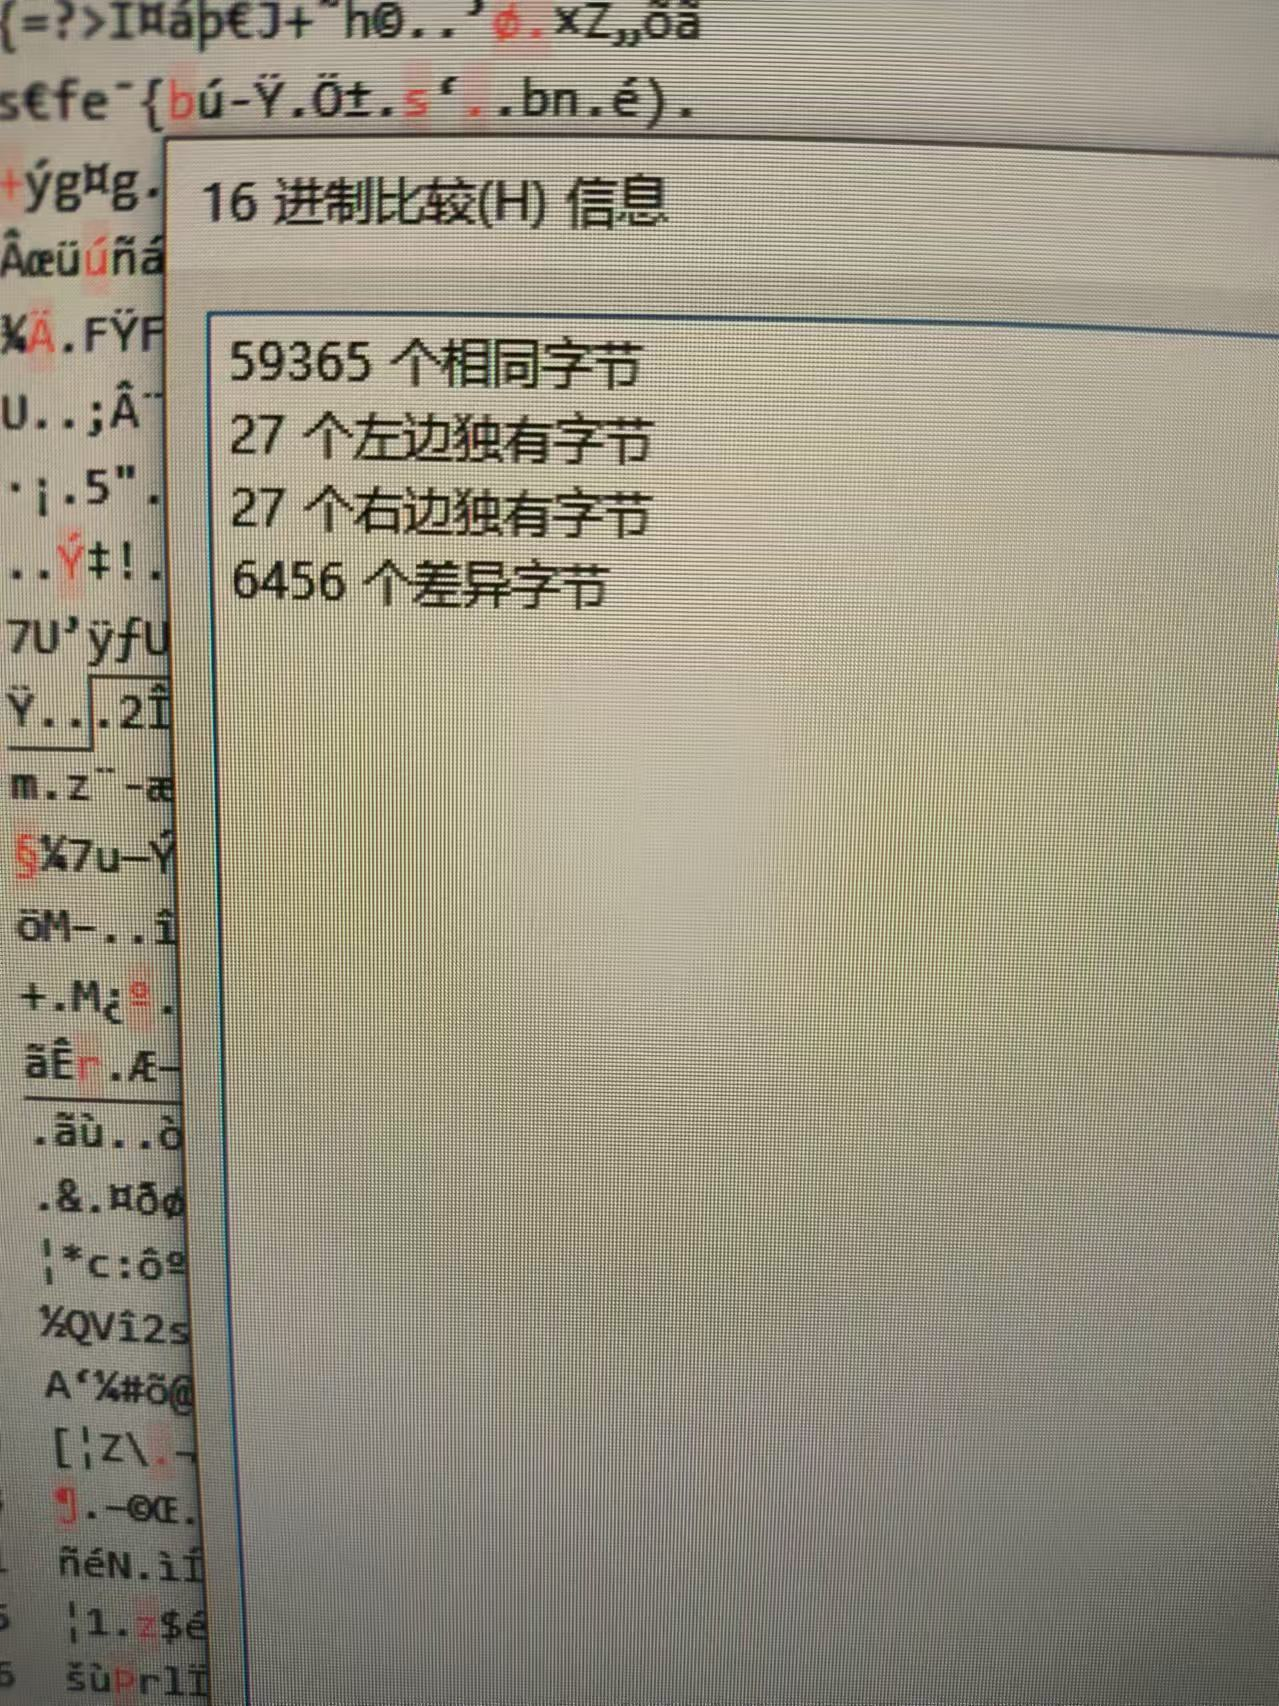
\includegraphics[width=0.4\textwidth]{D3-4-1.jpg}
				\caption{16进制比较信息}
				\label{fig:D3-4-1}
			\end{figure}

			\begin{table}[htbp]
				\centering
				\begin{tblr}{
				cells = {c},
				vline{1-3,5} = {-}{},
				hline{1-2,6} = {-}{},
				}
				序号 & 名称              & 数据       & 单位     \\
				1  & QKD 系统软件统计密钥率   & 37449.14 & bits/s \\
				2  & QKD 系统软件统计误码率   & 1.2      & \%     \\
				3  & QKD 系统误码估计采样率   & 10       & \%     \\
				4  & 手动误码率计算时所得数据误码率 & 1.23     & \%     
				\end{tblr}
				\caption{密钥分发过程数据处理实验数据记录表}
				\label{tbl:D3-4-1}
			\end{table}


	\subsection{实验过程中遇到的问题记录}

		\begin{enumerate}
			\item 由于使用的是高功率激光,一定要佩戴对应波长(404nm)的护目镜。
			\item 在调整光路时,注意所有光学元件应当保持等高共轴。
			\item 在使用手持功率探测器时,注意要让激光完全打在感光区域。
				
		\end{enumerate}



\subsection{实验数据记录}

	见\cref{fig:data}

	\begin{figure}[htbp]
		\centering
		% 第一行的三张图片
		\subfloat[原始数据1]
		{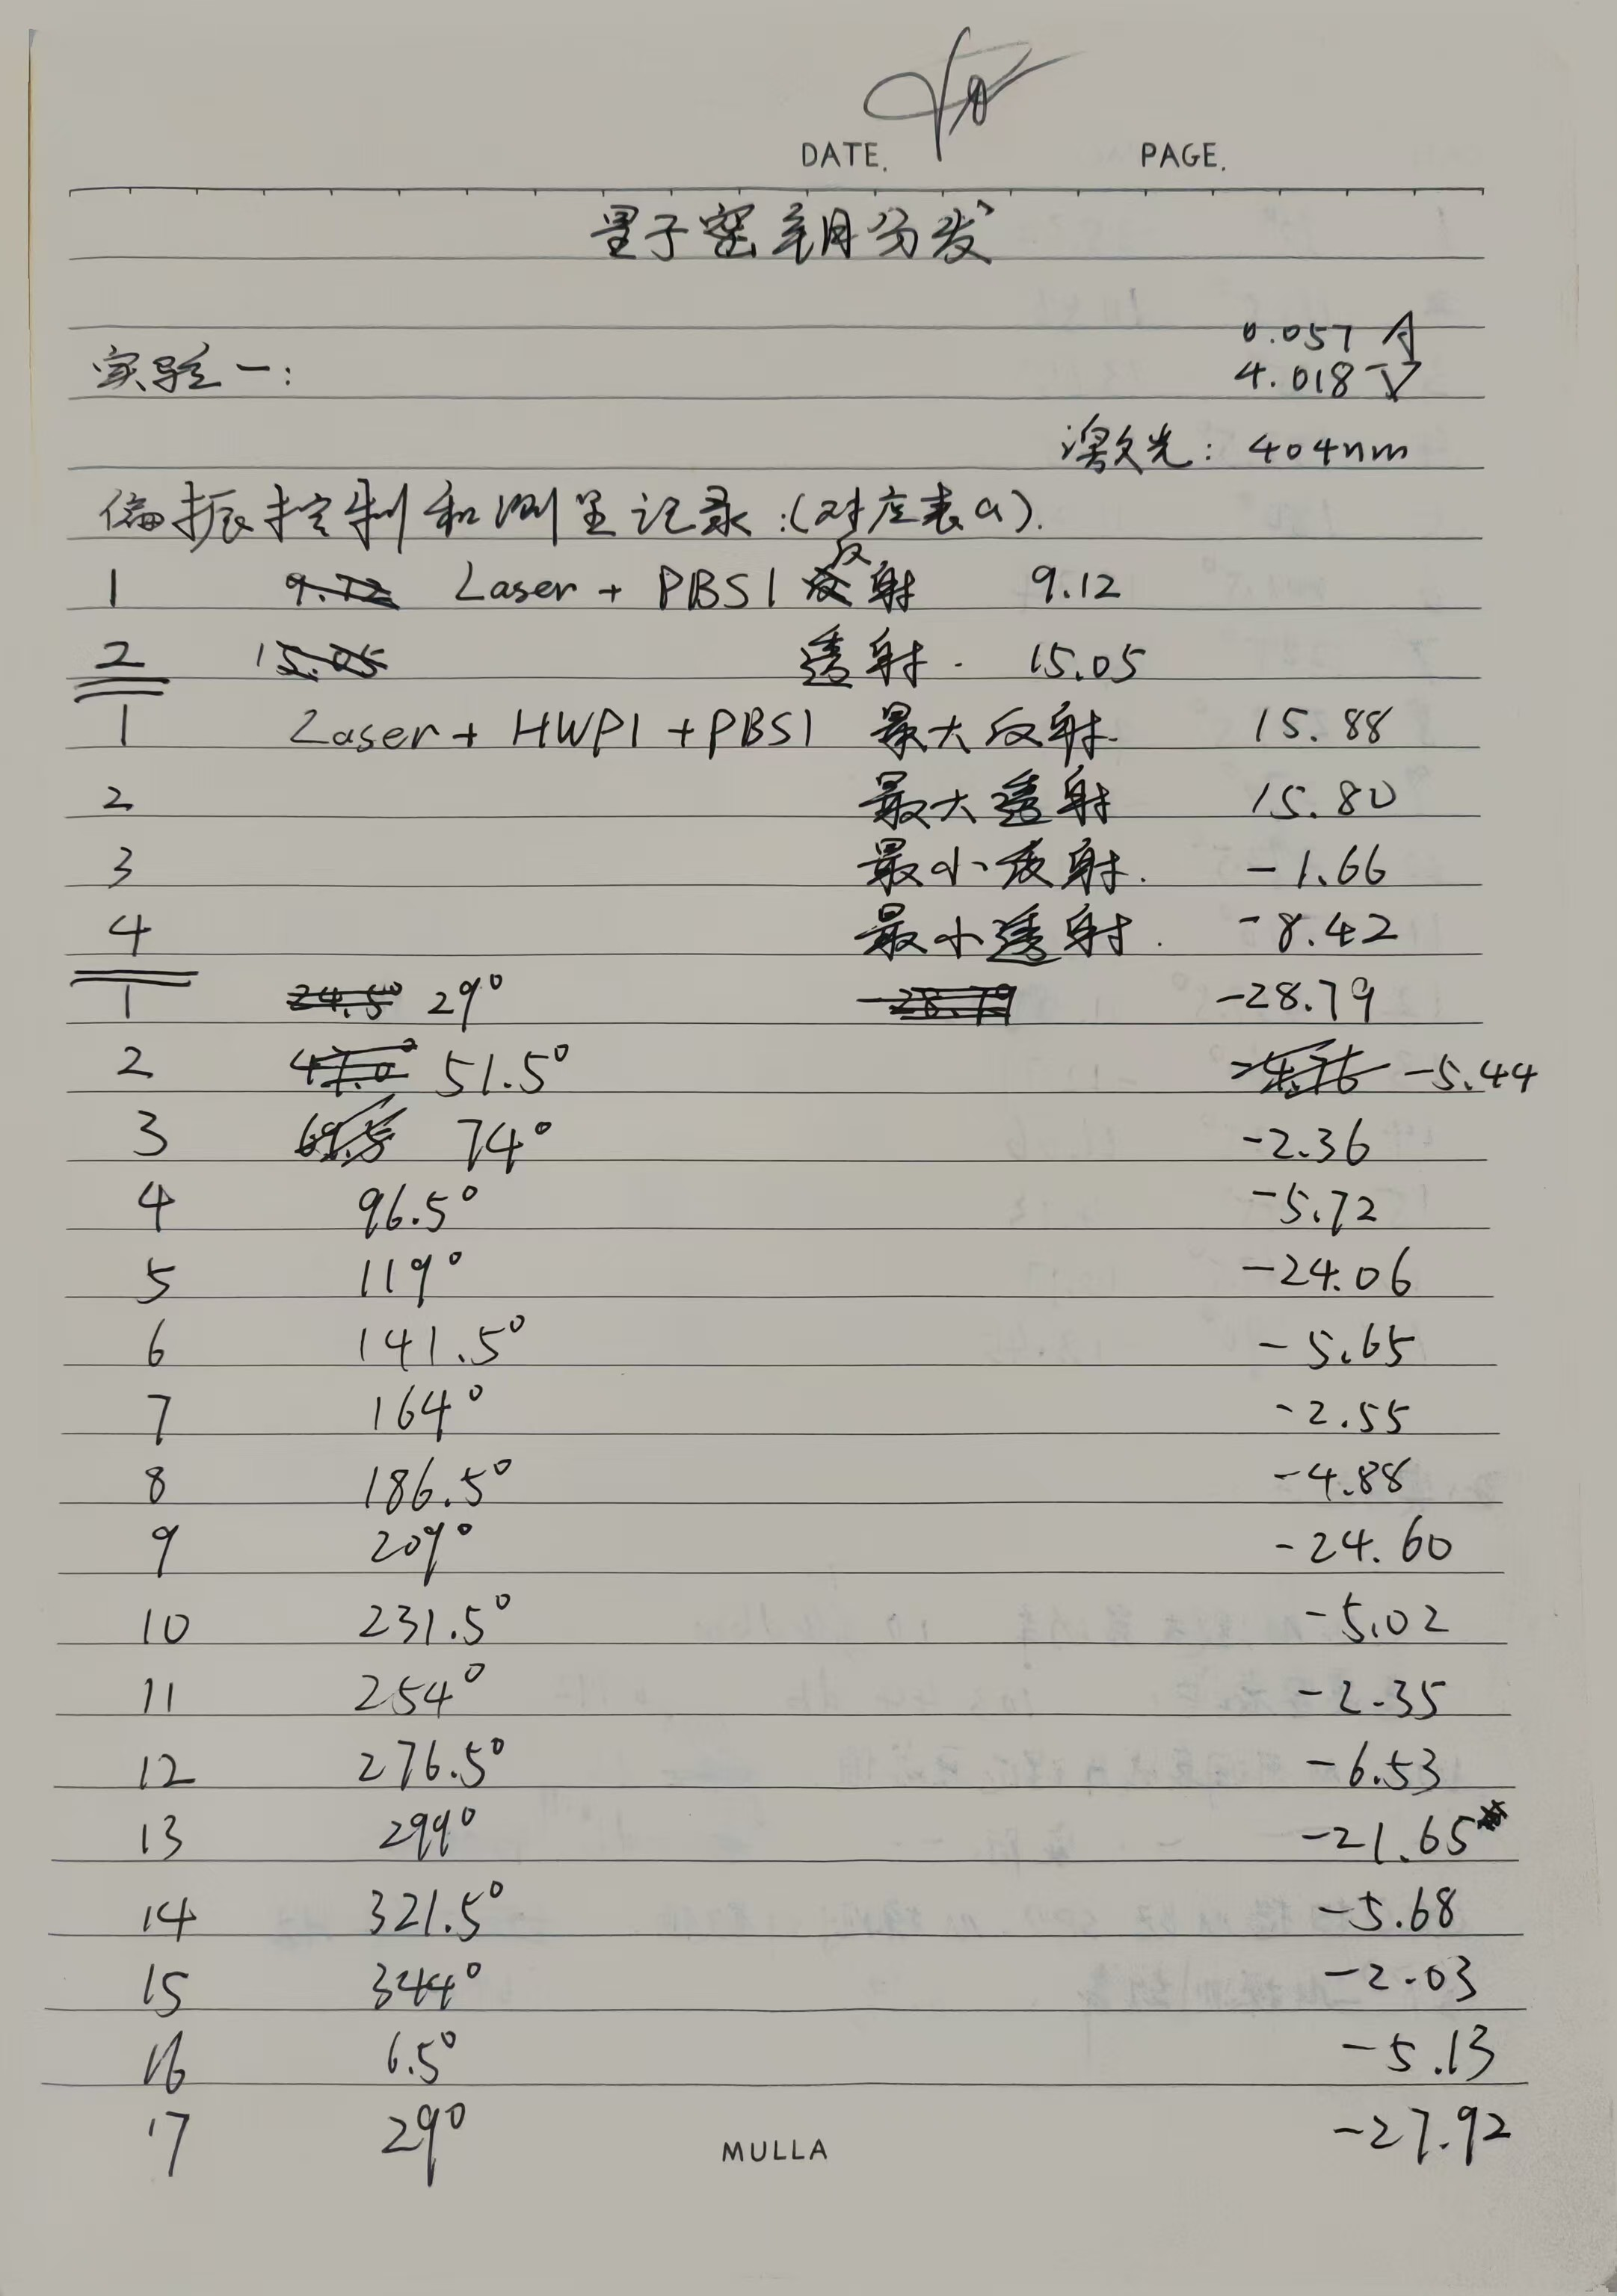
\includegraphics[width=0.3\textwidth]{D3-OriginalData-1.jpg}\label{fig:data1}}
		\quad
		\subfloat[原始数据2]
		{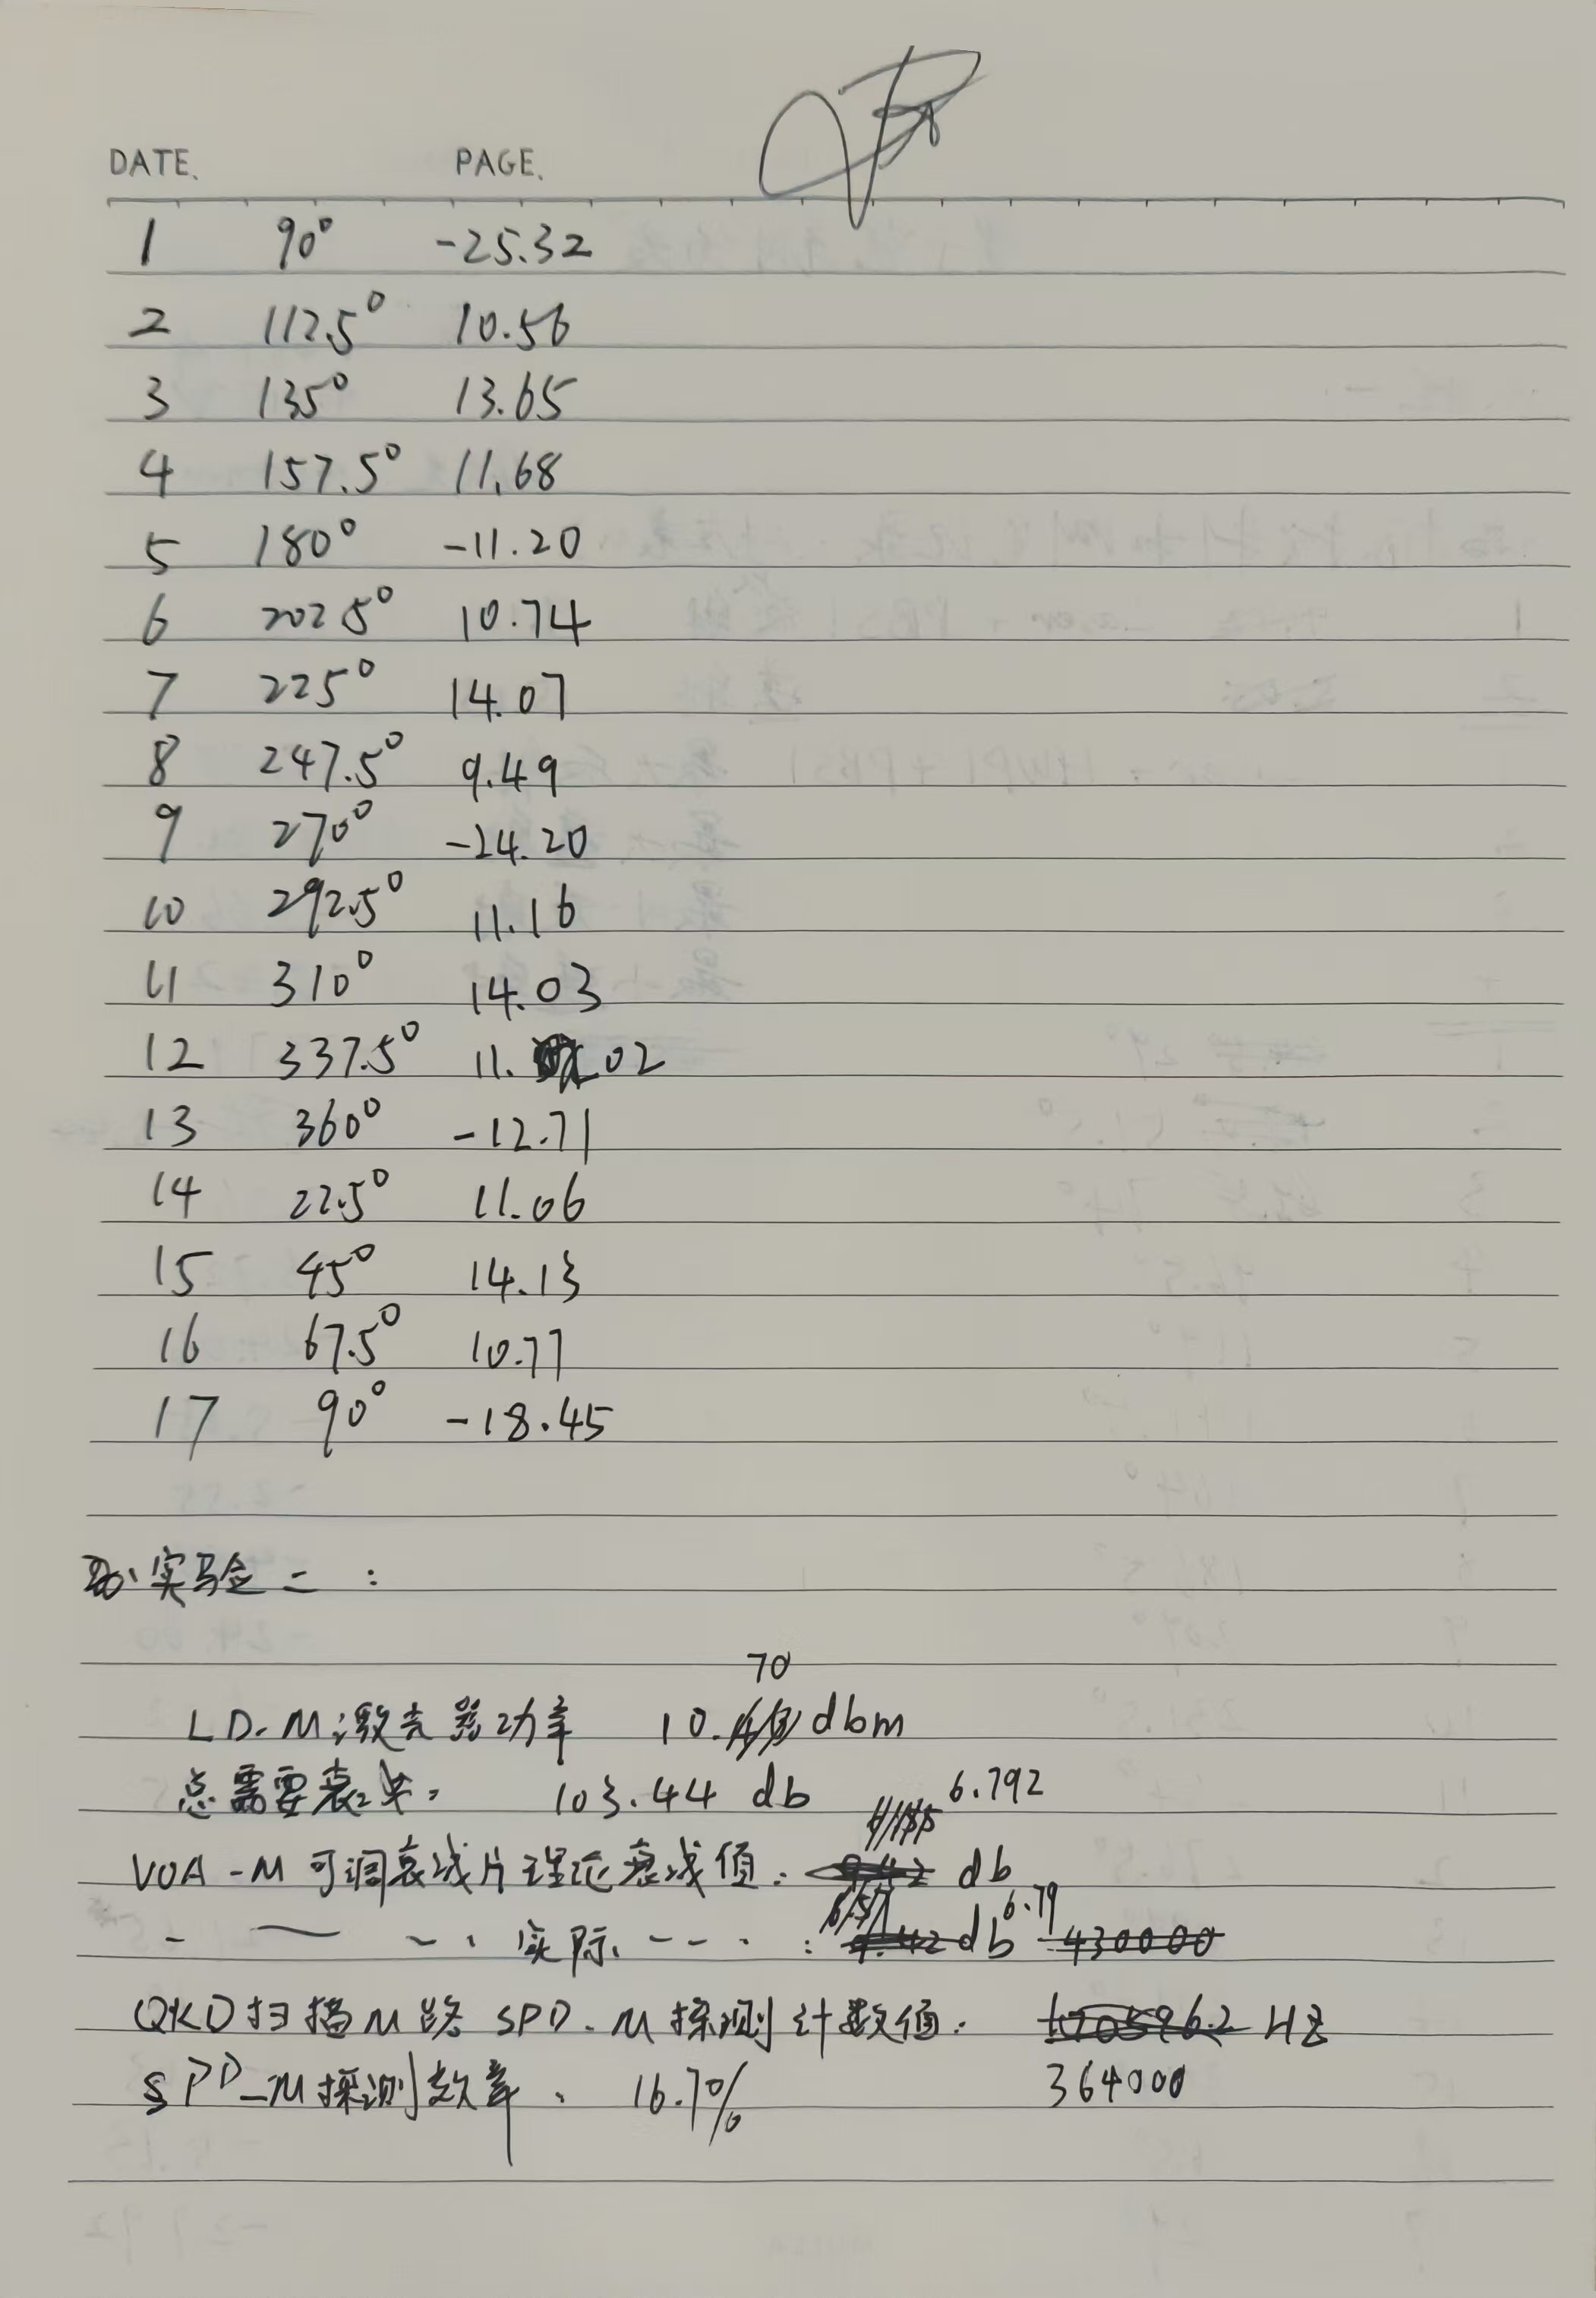
\includegraphics[width=0.3\textwidth]{D3-OriginalData-2.jpg}\label{fig:data2}}
		\quad
		\subfloat[原始数据3]
		{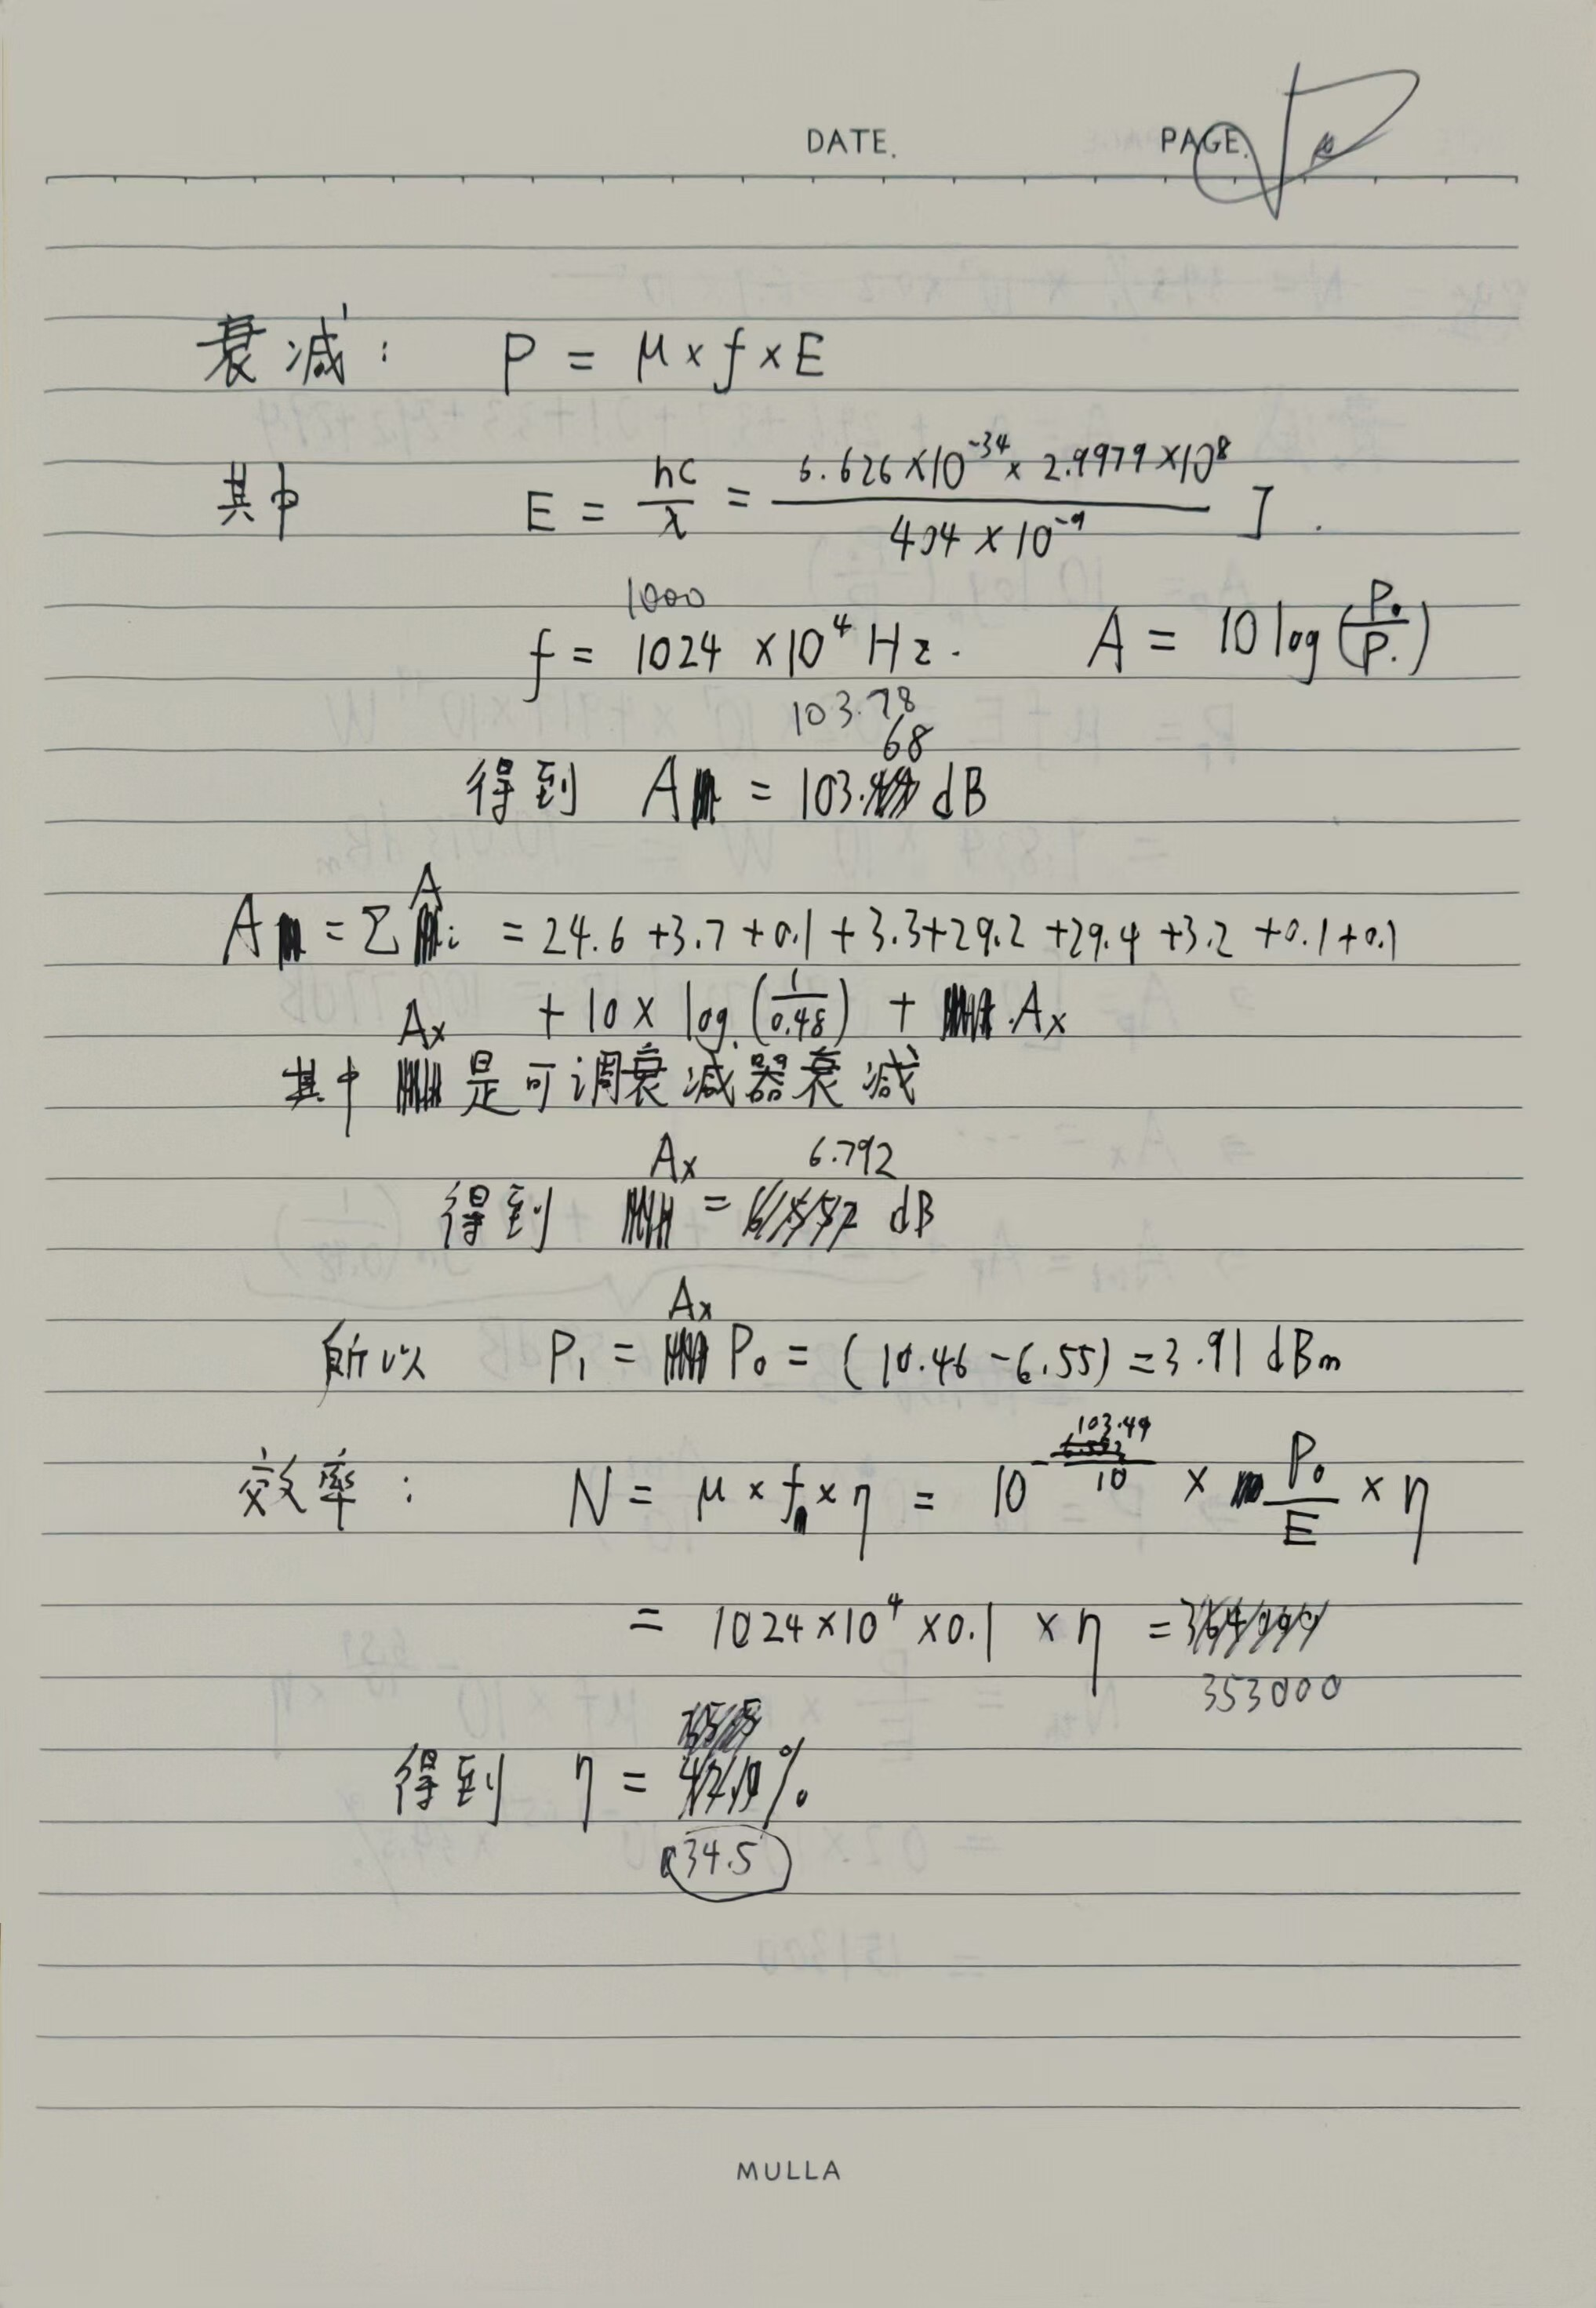
\includegraphics[width=0.3\textwidth]{D3-OriginalData-3.jpg}\label{fig:data3}}
		\newline
		% 第二行的两张图片
		\subfloat[原始数据4]
		{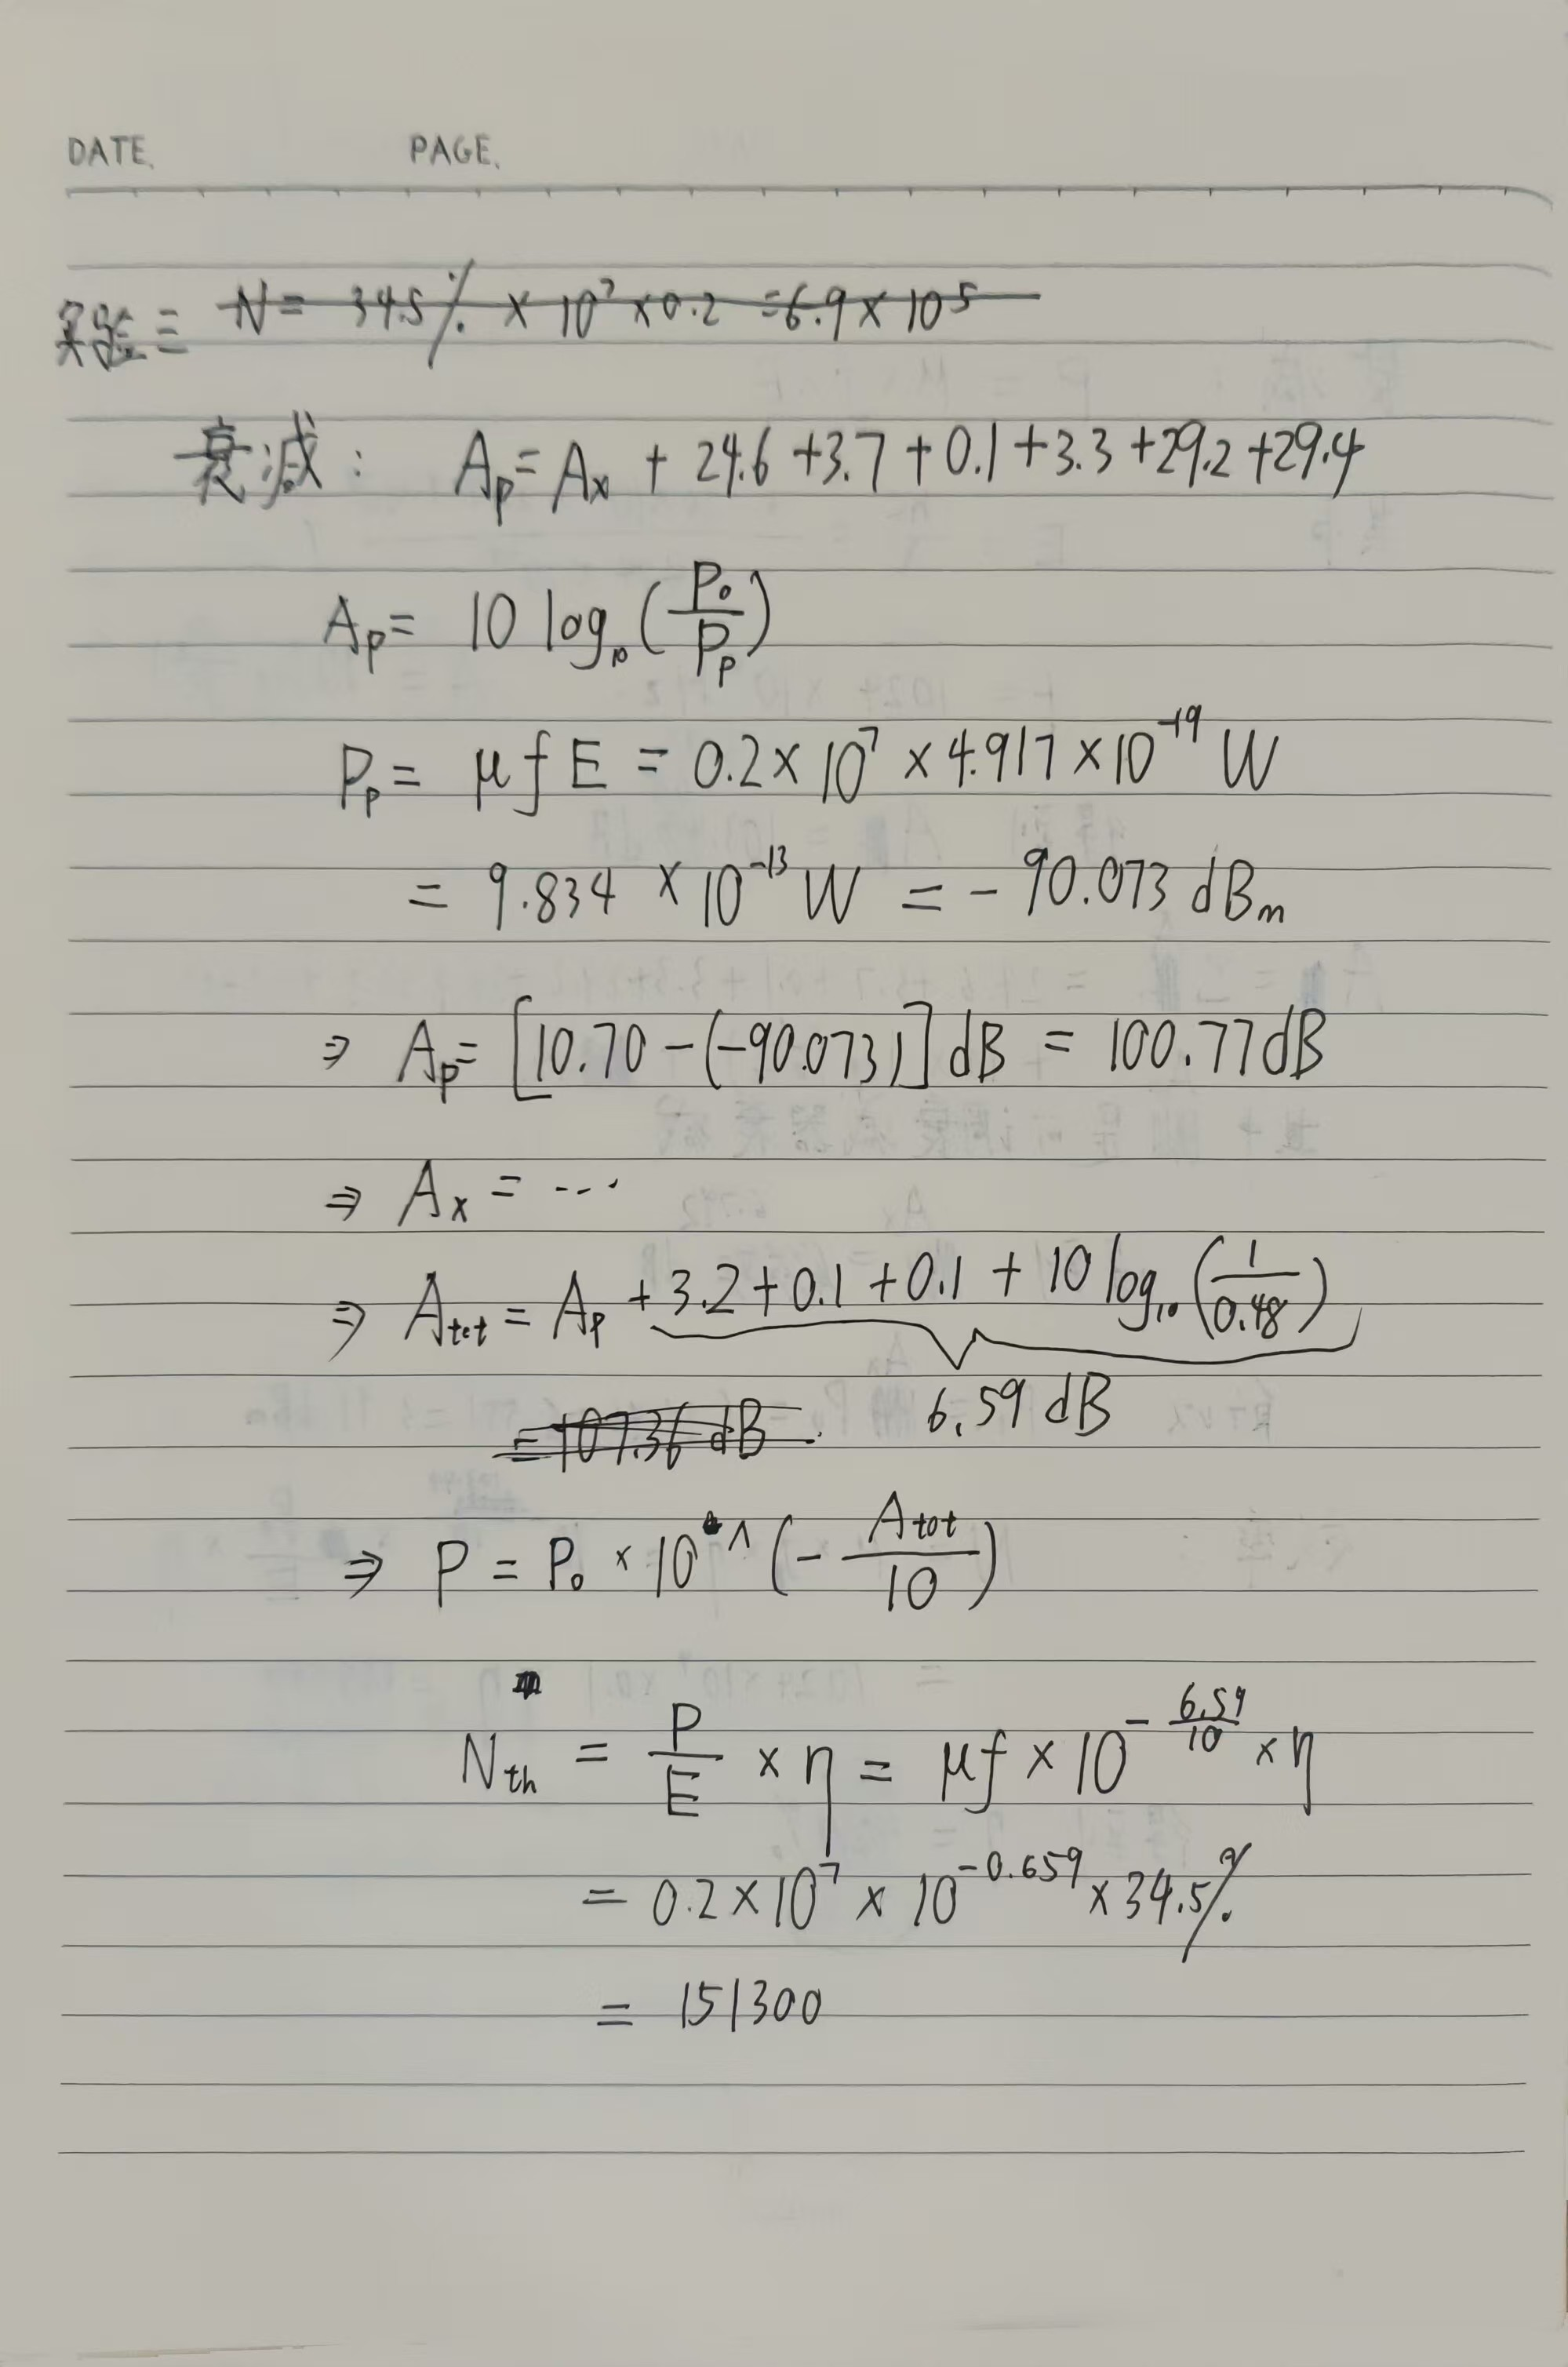
\includegraphics[width=0.3\textwidth]{D3-OriginalData-4.jpg}\label{fig:data4}}
		\quad
		\subfloat[原始数据5]
		{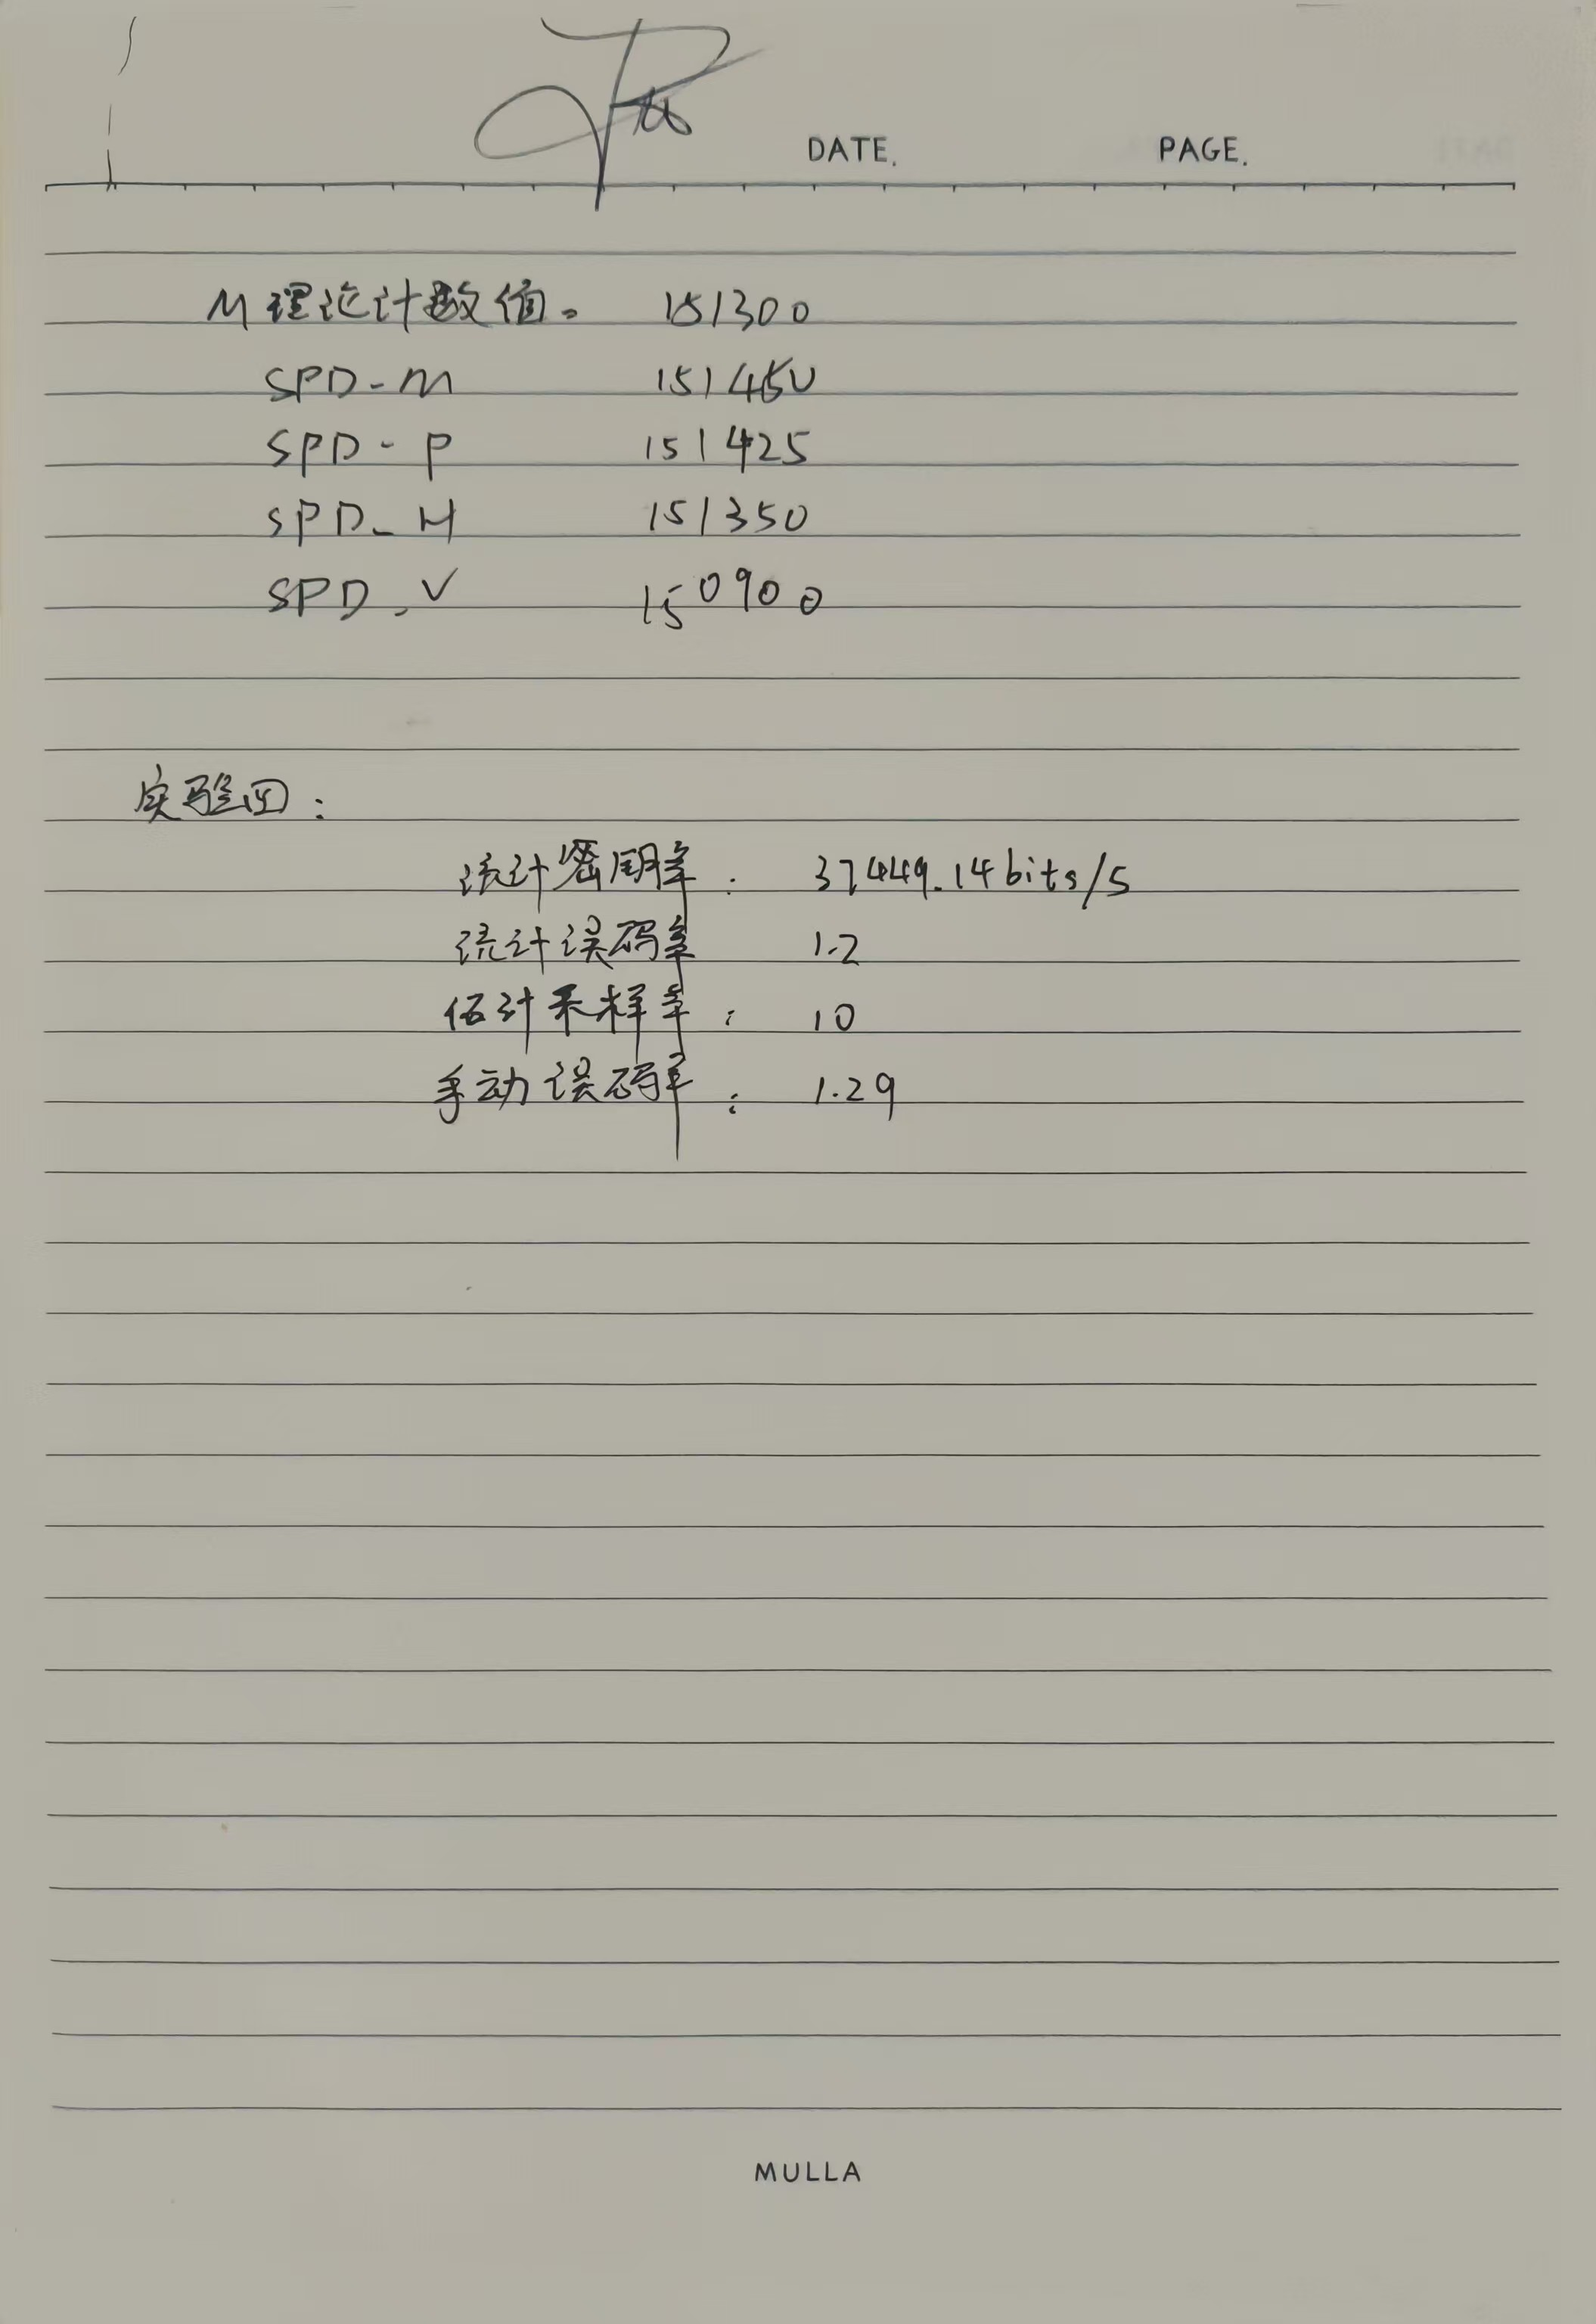
\includegraphics[width=0.3\textwidth]{D3-OriginalData-5.jpg}\label{fig:data5}}
		\caption{原始数据}
		\label{fig:data}
	\end{figure}
	



%\subsection{原始数据记录}


% \clearpage

	

\clearpage
\begin{table}
	\renewcommand\arraystretch{1.7}
	\begin{tabularx}{\textwidth}{|X|X|X|X|}
	\hline
	专业:& 物理学 &年级:& 2022级\\
	\hline
	姓名: & 戴鹏辉 & 学号:& 22344016\\
	\hline
    日期:& 2024/10/10 & 评分: &\\
	\hline
	\end{tabularx}
\end{table}

\section{D3 \quad 量子密钥分发 \quad\heiti 分析与讨论}

\subsection{实验数据分析}


	\subsubsection{实验一 \quad 光的偏振的测量和控制}

		对于偏振分光棱镜(PBS),它是一个分光棱镜,根据光的偏振态进行分光,当一束光垂直入射面入射,水平分量的光将会透射,垂直分量的光将会反射;即透射端口为水平偏振光,反射端口为垂直透射光。
		
		\begin{enumerate}
			\item 首先测量了激光通过 PBS1 后的反射和透射功率,如\cref{tbl:D3-1-1}所示,下面计算“假设其是线偏振光,其偏振方向与水平方向的夹角$\theta$”:
				% \begin{align*}
				% 	\text{设该线偏振光的光场为} \ \vec{E} = E_0 \cos\theta \vec{e_x} + E_0 \sin\theta \vec{e_y}	\\
				% 	\text{透射功率与反射功率之比为} \ \frac{P_t}{P_r} = \frac{(E_0 \cos\theta)^2}{(E_0 \sin\theta)^2} = \cot^2\theta = \frac{10^{\frac{15.05}{10}}}{10^{\frac{9.12}{10}}} = 3.9174		\\
				% 	\Rightarrow \theta = 0.468 \mathrm{rad}
				% \end{align*}

				\begin{align}
					\text{设该线偏振光的光场为} \ & \vec{E} = E_0 \cos\theta \vec{e_x} + E_0 \sin\theta \vec{e_y} \nonumber \\
					\text{透射功率与反射功率之比为} \ & \frac{P_t}{P_r} = \frac{(E_0 \cos\theta)^2}{(E_0 \sin\theta)^2} = \cot^2\theta = \frac{10^{\frac{15.05}{10}}}{10^{\frac{9.12}{10}}} = 3.9174 \nonumber \\
					& \Rightarrow \theta = 0.468 \, \mathrm{rad} \nonumber
				\end{align}

			即该偏振光与水平方向的夹角为 0.468 rad.

			\item 在“Laser”和“PBS1”之间加入一个半波片“HWP1”,旋转HWP1,测量激光器通过PBS1后的最大、最小透射功率和最大、最小的反射功率,结果如\cref{tbl:D3-1-2}所示,下面分析其是否为完美的线偏振光:
				\begin{itemize}
					\item 若其是线偏振光,在经过 HWP1 、旋转HWP1,后,其反射功率和透射功率应呈现周期性变化:
					
					设该线偏振光的光场为 
					$$ \vec{E} = E_0 \cos\theta \vec{e_x} + E_0 \sin\theta \vec{e_y} = E_0
					\begin{pmatrix}
						\cos\theta	\\
						\sin\theta
					\end{pmatrix} 
					$$

					设半波片的琼斯矩阵如下所示,其中$\alpha$为半波片光轴与水平方向的夹角 
					$$ \begin{pmatrix}
					 		\cos2\alpha		&\sin2\alpha	\\
							\sin2\alpha		&-\cos2\alpha
					 	\end{pmatrix} 
					$$

					当半波片作用在线偏振光后,有
					$$
						\vec{E'} = E_0 
						\begin{pmatrix}
							\cos2\alpha		&\sin2\alpha	\\
						   \sin2\alpha		&-\cos2\alpha
						\end{pmatrix}
						\begin{pmatrix}
							\cos\theta	\\
							\sin\theta
						\end{pmatrix} 
						= 
						\begin{pmatrix}
							\cos(2 \alpha - \theta)		\\
							\sin(2 \alpha - \theta)
						\end{pmatrix}
					$$

					所以,反射功率 $P_r = E_0^2 \cos^2(2 \alpha - \theta)$,透射功率 $P_t = E_0^2 \sin^2(2 \alpha - \theta)$

					即反射功率和透射功率都是周期性变化;且反射功率最大时,透射功率最小,反射功率最小时,透射功率最大;且最大反射光功率等于最大透射功率,最小反射功率等于最小透射功率。

					\item 由\cref{tbl:D3-1-2}所示,最小反射功率和最小透射功率之间差距较大,但都较小,可以认为是0,近似认为二者相等。两者差距较大可能是因为反射光与透射光受到不同方向的环境背景噪声的影响。
					
					但是最大反射功率和最大投射功率有$ P_{r,max} \approx P_{t,max} $,说明在高功率下,不同方向的环境背景噪声的影响可忽略不计。

					\item 综上所述,可认为其实完美的线偏振光。

				\end{itemize}

			
			\item 激光器后依次放置 PBS1,HWP1 和 PBS2。转动 HWP1 的角度 360 度,记下转动
			不同角度时,PBS2 出射端的功率变化,数据如\cref{tbl:D3-1-3}所示。

			由上面的计算,线偏振光经过半波片后的透射功率应满足公式 $P_t = E_0^2 \sin^2(2 \alpha - \theta)$,下面使用公式$ P_t = P_0 \sin^2(2\alpha - \theta) + C $对\cref{tbl:D3-1-3}进行拟合,图像如\cref{fig:D3-1-1}。

			由于$R^2 = 0.9816$,说明实验数据相当符合理论公式。

			由于我们将 半波片刻度的 29° 定义为数据列中的 0°,该刻度即为半波片的光轴。

			\begin{figure}[H]
				\centering
				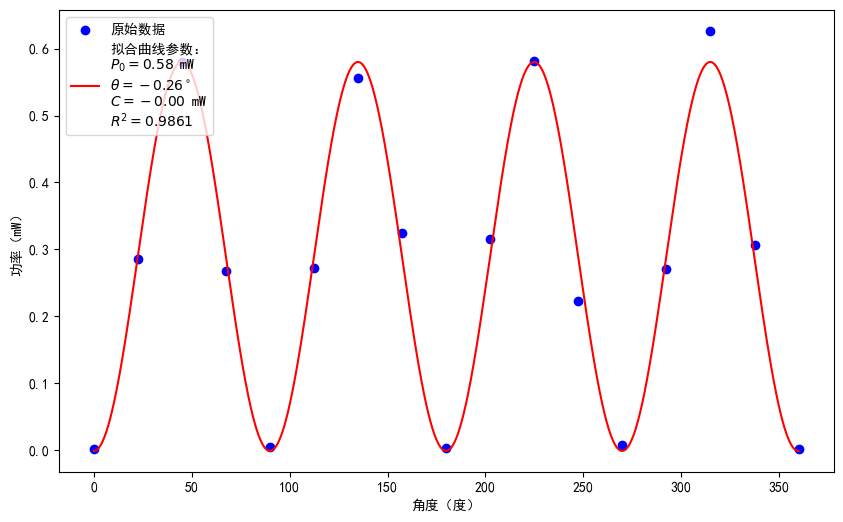
\includegraphics[width=0.9\textwidth]{D3-1-1.png}
				\caption{步骤3透射功率与理论计算拟合}
				\label{fig:D3-1-1}
			\end{figure}



			\item 使用上述 \cref{fig:D3-1-2} 的实验装置,将 HWP1 的角度调至光轴位置来制备偏振态 D(或与态D 垂直的态)。转动 HWP2,记录透过 PBS2 的光功率随着 HWP2 角度的变化。 

			由于此时 HWP1 的角度已调至光轴位置,所以经过 HWP1 的光已经是与水平方向45° 夹角的线偏振光(D态)。此时若 HWP2 的光轴设置至与水平方向 22.5° 夹角,D态将被旋转至水平方向偏振或竖直方向偏振。
			
			即经过 PBS2 的透射功率会达到最大或最小。若确实达到了最大或最小,说明 PBS2 之前的光确实在 D 态,具体拟合图像如\cref{fig:D3-1-3}所示。

			\begin{figure}[H]
				\centering
				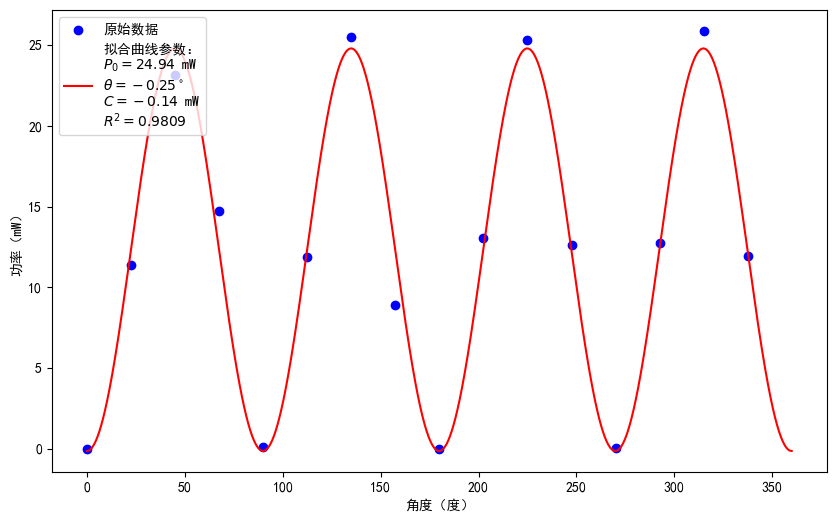
\includegraphics[width=0.9\textwidth]{D3-1-3.png}
				\caption{步骤4透射功率与理论计算拟合}
				\label{fig:D3-1-3}
			\end{figure}
			
		\end{enumerate}

			
















	\subsubsection{实验二 \quad 单光子的探测及相应探测器效率的测量}

		相关理论计算和单光子探测器的探测效率已在\cref{subsection2.1.2}中展示


	\subsubsection{实验三 \quad 单光子的标定}

		相关理论计算和单光子标定工作已在\cref{subsection2.1.3}中展示



	\subsubsection{实验四 \quad 密钥分发过程数据处理}


		由\cref{fig:D3-4-1}可知,使用软件进行文本比较的结果为:
			\begin{align}
				\text{相同字节数:} 59365	\nonumber\\
				\text{左边独有字节数:} 27	\nonumber\\
				\text{右边独有字节数:} 27	\nonumber\\
				\text{差异字节数字节数:} 6456	\nonumber
			\end{align}
			
		由于软件存储的格式为16进制,所以基于这些数据计算得到的为16进制下的误码率。

		记16进制格式的密钥误码率为$p_{16}$,2进制格式的密钥误码率为$p_{2}$。由于2位16进制数对应8位二进制数,且考虑到二进制文件误码率较小,所以两种格式的误码率存在如下关系:
		\[
			p_{16} = 1 - (1 - p_{2})^8 \approx 1 - (1 - 8p_{2}) = 8p_{2}
		\]
		其中,16进制误码率结果为:
		\[
			p_{16} = \frac{27 + 6456}{59365 + 27 + 6456} = 9.8454 \%
		\]
		所以,可估算2进制误码率为:
		\[
			p_{2} = \frac{p_{16}}{8} = 1.23 \%
		\]

		与软件直接给出的误码率 1.2\% (如\cref{tbl:D3-4-1}) 之间有一定误差,但作为一个误码率的估算已足够精确。

	
\subsection{实验后思考题}

% 思考题1
\begin{question}
	是否可以通过直接衰减任意的光源(比如白炽灯)的强度到单光子级别来得到真正的单光子源?(真正的单光子源是指每次触发可以确定性的得到一个仅包含一个光子的光脉冲信号)
\end{question}

	通过直接衰减白炽灯等传统光源的强度到非常低的水平,虽然可以减少发出的光子的平均数量,但这并不能得到真正的单光子源。原因在于传统光源(如白炽灯、激光器等)发出的光通常是经典的光场,其光子统计性质遵循泊松分布或更复杂的统计分布。即使将光源衰减到单光子级别,发出的光仍然可能包含多个光子,或者在某些时间点没有光子发射,因此无法确定性地产生每次只有一个光子的信号。

	真正的单光子源要求每次触发事件时只发射一个且仅一个光子,这种确定性发射通常需要量子光学手段来实现。比较常见的单光子源实现方法包括:
	\begin{enumerate}
		\item 量子点单光子源:量子点是一种半导体纳米结构,当其受到激发时,可以通过量子化的能级结构发射单个光子。
		\item 原子或离子系统:通过控制单个原子或离子的量子态来精确发射一个光子。
		\item 自发参量下转换(SPDC):虽然SPDC本质上是概率性的,但它可以通过条件测量技术,在检测到一个光子时,保证其伴随光子是单光子。
	\end{enumerate}

	这些方法都能够在量子层面精确控制光子的产生,而不是依赖于经典光源的统计衰减。因此,简单地通过衰减传统光源的强度不能产生真正意义上的单光子源。







% 思考题2
\begin{question}
	了解单光子探测器暗计数的原理,并设计实验装置测量探测器的暗计数率。
\end{question}



	单光子探测器的暗计数是指探测器在没有实际接收到光子的情况下产生的错误计数。暗计数主要由热噪声、宇宙射线、放射性材料的辐射等随机噪声源引起。暗计数会影响探测器的精度,尤其是在单光子级别的实验中,了解和测量暗计数率是非常重要的。

	\begin{enumerate}
		\item \textbf{暗计数的工作原理}:
			单光子探测器(如光电倍增管、硅光电倍增器、超导纳米线单光子探测器等)在工作时会受到各种外部和内部噪声的影响,即使在完全黑暗的条件下,探测器也可能由于这些噪声产生错误的信号,称为暗计数。这些暗计数的频率可以通过一定时间内记录到的无光信号的计数来估算。

		\item \textbf{实验装置设计测量探测器的暗计数率}
			\begin{itemize}
				\item \textbf{光源控制:}
					确保探测器处于完全黑暗的环境中,以便排除任何来自外部光子的干扰。你可以将探测器放置在一个不透光的封闭盒子中,或者使用特制的屏蔽设备。

				\item \textbf{探测器设置:}
					选择合适的单光子探测器,常见类型包括光电倍增管(PMT)、雪崩光电二极管(APD)或超导纳米线单光子探测器(SNSPD)。不同类型的探测器有不同的暗计数率,因此应了解其基本特性。
					
					调节探测器的偏压或增益设置到推荐工作区域,以确保其正常工作。

				\item \textbf{数据采集:}
					将探测器与计数系统(如数字示波器或计数模块)相连,以记录探测器的输出信号。

					设定合适的时间窗口,记录在一段时间内(如几分钟)的探测器输出信号。在此过程中不应打开光源。

					记录下所有的信号输出,即这些信号都视为暗计数。

				\item \textbf{计算暗计数率:}
					将记录到的总暗计数除以测量的总时间,计算单位时间内的暗计数率:
					\[
						\text{暗计数率} = \frac{\text{暗计数的总数}}{\text{测量时间(秒)}}
					\]

			\end{itemize}
	\end{enumerate}







% 思考题3
\begin{question}
	量子密钥分发实验中对基后的数据,为什么会有误码出现,如何降低误码?
\end{question}

	误码出现的原因:
	\begin{enumerate}
		\item \textbf{量子态传输中的噪声:}
			在QKD过程中,量子态(如光子)的传输通常通过光纤或自由空间。由于环境噪声、光纤损耗、干扰以及光子检测器的噪声,接收端可能无法精确还原发送端的量子态,导致误码。

		\item \textbf{探测器效率和暗计数:}
			单光子探测器并非完美的设备,它们在检测信号时可能会因为效率问题漏掉光子,或者因为暗计数引入额外的误码。这种探测器本身的误差会导致接收到的量子态与发送端不一致。

	\end{enumerate}

	降低误码率的措施:
	\begin{enumerate}
		\item \textbf{提高探测器性能:}
			使用更高效率的单光子探测器,减少暗计数率(错误计数)和探测效率低的问题。例如,超导纳米线单光子探测器(SNSPD)具有较低的暗计数和较高的检测效率。

		\item \textbf{降低量子态传输中的噪声:}
			优化量子信道的传输条件,如通过更高质量的光纤减少信号衰减或使用更好的光学元件减少信号失真。
		
			对于自由空间传输,选择合适的天气和传输路径,以避免环境噪声和干扰的影响。

		\item \textbf{纠错算法:}
			在基后的数据处理中,使用经典的纠错编码算法(如Cascade、LDPC等)来修正传输中的误码。纠错可以在保证数据安全的前提下修复小概率的错误,从而降低误码率。
	\end{enumerate}


\clearpage
\section{D3 \quad 量子密钥分发 \quad\heiti 实验总结}

	\subsection{实验分工}

		本次实验由戴鹏辉、杨舒云、马万成、朱政鑫四名同学共同完成。

		实验数据记录由杨舒云同学完成。

		实验理论计算由朱政鑫同学完成。

		实验操作由戴鹏辉和马万成同学完成。


	\subsection{实验心得}

	\begin{figure}[H]
		\centering
		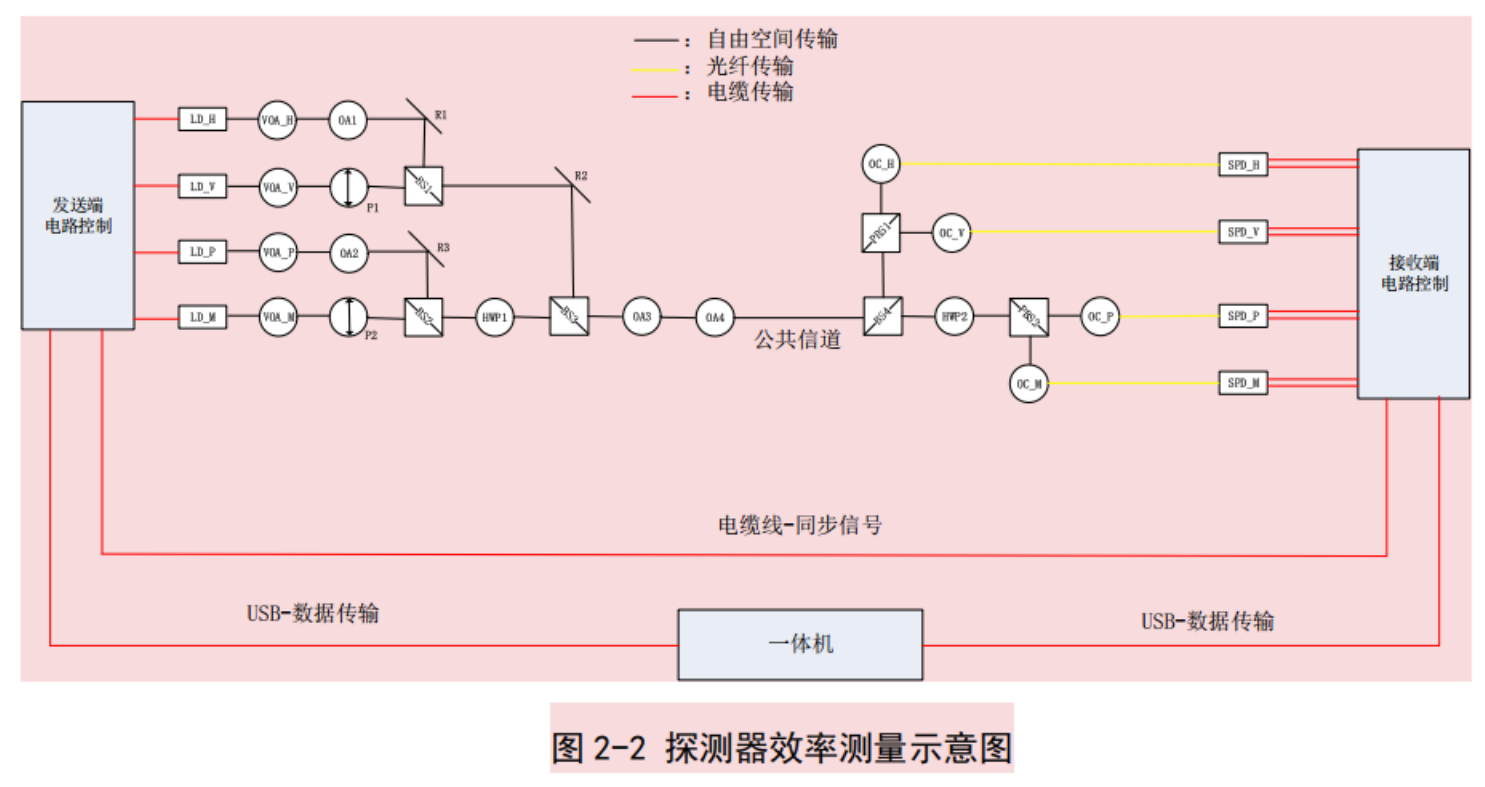
\includegraphics[width=0.9\textwidth]{D3-Sum-1.png}
		% \caption{步骤4透射功率与理论计算拟合}
		\label{fig:D3-1-3}
	\end{figure}

	在实验结束时,老师问我们,BS4的作用是什么。现在将我对该元件的理解写在这里。

	在公共信道处的光子可能存在4中偏振态,即H、V、P、M。当光子到达 BS4 时,会随机的被反射或者折射。
	\begin{enumerate}
		\item 如果被反射(即向上走),那么又有两种可能,光子是 H 或 V 态之一,或者是 P 或 M 态之一。
			\begin{itemize}
				\item 如果光子是 H 或 V 态之一,那么经过 PBS1 后,H态的光子会直接透射,不可能被反射;V态的光子会直接被反射,不可能被透射,即路径是确定的。
				\item 如果光子是 P 或 M 态之一,那么在经过 PBS1 后,其路径依然无法确定。
			\end{itemize}
		
		\item 如果光子透射,那么同样有两种可能,光子是 H 或 V 态之一,或者是 P 或 M 态之一。
		\begin{itemize}
			\item 如果光子是 P 或 M 态之一,那么在经过 HWP2 后,其偏振方向将会被旋转至水平或垂直方向,随后经过 PBS2 ,其路径是确定的
			\item 如果光子是 H 或 V 态之一,那么在经过 HWP2 后,原本水平或垂直方向的偏正将会被旋转,那么经过 PBS2 后,其路径将不再确定。
		\end{itemize}
	\end{enumerate}

	综上所述,BS4 的作用即随机的选择 $\oplus$ 和 $\otimes$ 基进行测量,若光子被反射,即选择了$\oplus$ 基进行测量;若光子透射,即使用了$\otimes$基进行测量。使用与光子偏振态相符的基测量,能够保证光子的路径确定,其偏振态的测量也是确定且正确的。
	


\end{document}
